% Modelo de Trabalho Acadêmico da UNESP de Guaratinguetá v-1.0
% Copyright 2017 by Eduardo Rohde Eras
%
% This program is free software: you can redistribute it and/or modify
% it under the terms of the GNU General Public License as published by
% the Free Software Foundation, either version 3 of the License, or
% (at your option) any later version.
%
% This program is distributed in the hope that it will be useful,
% but WITHOUT ANY WARRANTY; without even the implied warranty of
% MERCHANTABILITY or FITNESS FOR A PARTICULAR PURPOSE.  See the
% GNU General Public License for more details.
%
% You should have received a copy of the GNU General Public License
% along with this program.  If not, see <http://www.gnu.org/licenses/>.

%----------------------------------------------------------------------------------------%
% C L A S S E   D O   D O C U M E N T O
%----------------------------------------------------------------------------------------%

\documentclass[
  %----------------------------------------------------------------------------------------%
  %Opções da classe 'memoir'
  %----------------------------------------------------------------------------------------%
  12pt,		% Tamanho da Fonte.
  a4paper,	% Tamanho da página.
  openright,% Capítulos começam em páginas ímpares (insere uma página vazia se necessário).
  oneside,	% Para impressão em frente e verso utilizar twoside.
  %----------------------------------------------------------------------------------------%
  %Opções da classe 'abntex2'
  %----------------------------------------------------------------------------------------%
  chapter=TITLE,		%Títulos de capítulos convertidos em letras maiúsculas.
  section=TITLE,		%Títulos de seções convertidos em letras maiúsculas.
  %----------------------------------------------------------------------------------------%
  %Opções da classe 'babel'
  %----------------------------------------------------------------------------------------%
  english,	%Idioma adicional para hifenização.
  french,	%Idioma adicional para hifenização.
  spanish,	%Idioma adicional para hifenização.
  brazil	%Idioma principal do documento.
  %----------------------------------------------------------------------------------------%
]{abntex2}

%----------------------------------------------------------------------------------------%
% P A C O T E S
%
% Insira aqui os pacotes que for utilizar em seu documento. Para saber quais pacotes o
% template já está utilizando, confira o arquivo "pacoteBasico.sty".
%----------------------------------------------------------------------------------------%
    
    \usepackage{pacoteBasico}   %Pacote Básico de formatação no padrão da UNESP/FEG
    \usepackage{color}		    %Controle das cores.
    \usepackage{graphicx}	    %Inclusão de gráficos.
    \usepackage{lipsum}		    %Para geração de 'Dummy Text'.
    \usepackage{afterpage}
    \usepackage{lscape}
    \usepackage{longtable}
    \usepackage{booktabs}
    
%----------------------------------------------------------------------------------------%
% I N F O R M A Ç Õ E S   B Á S I C A S   S O B R E   O   T R A B A L H O
%
% Defina aqui as informações pertinentes ao trabalho.
%----------------------------------------------------------------------------------------%

    %----------------------------------------------------------------------------------------%
    % D A D O S   P E S S O A I S
    %----------------------------------------------------------------------------------------%
    
    %Nome completo do autor do presente Trabalho de Graduação:
    \newcommand{\nomeDoAutor}{
    Matheus Cerqueira de Jesus
    }
    
    %Nome do curso em que o autor está se graduando:
    \newcommand{\nomeDoCurso}{
    Engenharia Elétrica
    }
    
    %----------------------------------------------------------------------------------------%
    % D A D O S   S O B R E   O   T R A B A L H O
    %----------------------------------------------------------------------------------------%
    
    %Título do presente trabalho:
    \newcommand{\tituloDoTrabalho}{
        Machine Learning para estimar o número de internações por doenças respiratórias em Cuiabá-MT
    }
    
    % Subtítulo do presente trabalho, se houver:
    % \newcommand{\subtituloDoTrabalho}{
    
    % }
    
    %Mês da entrega do trabalho
    \newcommand{\mesDeEntrega}{
    Fevereiro
    }
    
    %Ano da entrega do trabalho
    \newcommand{\anoDeEntrega}{
    2023
    }
    
    %----------------------------------------------------------------------------------------%
    % D A D O S   D O S   O R I E N T A D O R E S,   B A N C A   E   C O O R D E N A D O R
    %----------------------------------------------------------------------------------------%
    
    %Nome do orientador do presente trabalho:
    \newcommand{\nomeDoOrientador}{
    Paloma Maria Silva Rocha Rizol
    }
    
    %Título do orientador:
    \newcommand{\tituloDoOrientador}{
    Profº Dr.
    }
    
    %Nome do coorientador do presente trabalho:
    \newcommand{\NomeDoCoorientador}{
    Taynara de Oliveira Castellões
    }
    
    %Título do coorientador:
    \newcommand{\tituloDoCoorientador}{
    Eng.
    }
    
    %Nome do Coordenador do Curso:
    \newcommand{\nomeDoCoordenador}{
    Daniel Julien Barros da Silva Sampaio
    }
    
    %Título do coordenador do Curso:
    \newcommand{\tituloDoCoordenador}{
    Profº Dr.
    }
    
    %Nome do Membro Interno da Banca:
    \newcommand{\nomeDoMembroInterno}{
    Taynara de Oliveira Castellões
    }
    
    %Título do Membro Interno da Banca:
    \newcommand{\tituloDoMembroInterno}{
    Eng.
    }
    
    %Nome do membro Externo da banca:
    \newcommand{\nomeDoMembroExterno}{
    Leonardo Mesquita
    }
    
    %Título do Membro Externo da Banca:
    \newcommand{\tituloDoMembroExterno}{
    Profº Dr.
    }
    
    %----------------------------------------------------------------------------------------%
    % D A D O S   D A   I N S T I T U I Ç Ã O
    %----------------------------------------------------------------------------------------%
    
    %Nome da Universidade
    \newcommand{\nomeDaUniversidade}{
    Universidade Estadual Paulista "Júlio de Mesquita Filho"
    }
    
    %Nome da Cidade
    \newcommand{\nomeDaCidade}{
    Guaratinguetá
    }

%----------------------------------------------------------------------------------------%
% I N Í C I O   D O   D O C U M E N T O - P R É   T E X T U A L
%----------------------------------------------------------------------------------------%
\begin{document}
    
    \imprimircapa
    \imprimirfolhaderosto
    
    %------------------------------------------------------------------------------------%
    % F O L H A   D E   A P R O V A Ç Ã O
    %
    % OBRIGATÓRIO. Este é o modelo de folha de aprovação que deve ser digitalizada após as
    % assinaturas da banca. Utilize um software de edição de PDF para substituição posterior
    % dessa folha. Se possível, utilize um recurso de assinatura digital fornecido pela
    % ferramenta de edição de PDF, evitando assim a digitalização da folha toda.
    %------------------------------------------------------------------------------------%
    \begin{folhadeaprovacao}
        \begin{center}
        
        {\sffamily
            \bfseries{
                \Large{
                    UNIVERSIDADE ESTADUAL PAULISTA\par
                    "JÚLIO DE MESQUITA FILHO"\par
                }
            }
            CAMPUS DE GUARATINGUETÁ
        }
        
        \vspace*{3cm}
                
        \normalsize{\textbf{\MakeUppercase\nomeDoAutor}}
        
        \vspace*{1cm}
        
       % {\setstretch{1.0}
        \begin{framed}
            ESTE TRABALHO DE GRADUAÇÃO FOI JULGADO ADEQUADO COMO PARTE DO REQUISITO PARA A OBTENÇÃO DO DIPLOMA DE \textbf{"GRADUANDO EM {\MakeUppercase\nomeDoCurso}"}
            \par
            \vspace*{1cm}
            APROVADO EM SUA FORMA FINAL PELO CONSELHO DE CURSO DE GRADUAÇÃO EM {\MakeUppercase\nomeDoCurso}
            \par
            \vspace*{1cm}
            \begin{flushright}
            \tituloDoCoordenador {\MakeUppercase\nomeDoCoordenador}
            \par
            Coordenador
            \end{flushright}
       \end{framed}
      % }
       
       \begin{flushleft}
            \textbf{BANCA EXAMINADORA:}
       \end{flushleft}
       
       \assinatura{\small \tituloDoOrientador \nomeDoOrientador \par Orientador/UNESP-FEG}
       \assinatura{\small \tituloDoMembroInterno \nomeDoMembroInterno \par UNESP-FEG}
       \assinatura{\small \tituloDoMembroExterno \nomeDoMembroExterno \par UNESP-FEG}
       
       \vfill
       \mesDeEntrega, \anoDeEntrega
        
        \end{center}
    \end{folhadeaprovacao}
    
    %------------------------------------------------------------------------------------%
    % D A D O S   C U R R I C U L A R E S
    % 
    % OBRIGATÓRIO PARA PÓS-GRADUAÇÃO.
    % Inserir a data inicial e final de cada formação acadêmica. Para os alunos que não
    % precisarem de uma folha de dados curriculares em seu trabalho, basta apagar todo 
    % o código dessa seção.
    %------------------------------------------------------------------------------------%
    
    \begin{center}
        \normalsize{\textbf{\MakeUppercase{Dados Curriculares}}} \par
        \vspace*{1cm}
        \normalsize{\textbf{\MakeUppercase\nomeDoAutor}} \par
        \vspace*{1cm}
        
        \begin{tabular}{ l p{7cm} }
            \textbf{\MakeUppercase{Nascimento}} & 09/11/1999 - São José dos Campos / SP \\
            \\
            \textbf{\MakeUppercase{Filiação}} & Antonio Sergio de Jesus \\
            & Maria do Socorro Cerqueira de Jesus \\
        \end{tabular}
    \end{center}
    \newpage
    
    %------------------------------------------------------------------------------------%
    % D E D I C A T Ó R I A
    %
    % OPCIONAL. Se não for utilizar uma dedicatória, basta apagar todo o código dessa seção.
    %------------------------------------------------------------------------------------%
    
    \begin{dedicatoria}
        \vspace*{\fill}
        \begin{flushright}
            Dedico este trabalho à todos aqueles que assim como eu, 
            acreditam que a educação é a ferramenta mais poderosa na luta contra a opressão. 
        \end{flushright}
        \vspace*{1cm}
    \end{dedicatoria}

    %------------------------------------------------------------------------------------%
    % A G R A D E C I M E N T O S
    %
    % OPCIONAL. Citar as pessoas, instituição, agência de fomento, entre outros que contribuíram
    % de maneira relevante à elaboração do trabalho e na vida acadêmica.
    % Se não for utilizar os agradecimentos, basta apagar todo o código dessa seção.
    %------------------------------------------------------------------------------------%
    \begin{agradecimentos}
    
        Eu agradeço, primeiramente, aos meus pais que sempre acreditaram em mim, provendo todo o 
        suporte necessário para que eu alcance os meus objetivos.

        Agradeço a minha orientadora Paloma Maria Silva Rocha Rizol e coorientadora Taynara de Oliveira Castellões
        por todo o apoio durante o desenvolvimento desse trabalho.
        
        Agradeço aos professores e amigos
        Luis Rogerio de Oliveira Hein e Maurício de Oliveira Filho por todas as conversas e horas
        de trabalho juntos, vocês participaram da minha formação como pessoa. 
        
        Agradeço aos meus queridos amigos Tales Hiro Cardoso Ishida, Thales Vieira e Silva 
        Lobo De Almeida, Vinicius Mancini e Matheus Vinicius Resende Nascimento, 
        por todas as horas de estudo juntos e
        todos os bons momentos que tivemos.
        
        Agradeço a todos os professores e funcionários da universidade que contribuiram para a minha formação. 
        
        Finalmente, agradeço a minha companheira Deborah Eberle dos Santos por todo o incentivo, paciência,
        momentos felizes e por me fazer ser uma pessoa melhor.
    
    \end{agradecimentos}
    
    %------------------------------------------------------------------------------------%
    % F O M E N T O
    %
    % OBRIGATÓRIO PARA ALUNO BOLSISTA. Esta página contém informações sobre o financiamento
    % recebido para o desenvolvimento da tese/dissertação. Utilize o(s) nome(s) da(s) 
    % instituição(ões) que forneceu(ram) o auxílio financeiro para seu trabalho. Se não
    % for utilizar o fomento em seu trabalho, basta apagar todo o código dessa seção.
    %------------------------------------------------------------------------------------%
    % \vspace*{\fill}
    % \begin{flushleft}
    %     Este trabalho contou com o apoio da(s) seguinte(s) entidade(s):\\
    %     FAPESP - Fundação de Amparo à Pesquisa do Estado de São Paulo\\
    %     CAPES - Coordenação de Aperfeiçoamento de Pessoa de Nível Superior\\
    %     CNPq - Conselho Nacional de Desenvolvimento Científico e Tecnológico\\
    %     SIGQ - Sigla de Uma Instituição Genérica Qualquer
    % \end{flushleft}
    % \newpage
    
    %------------------------------------------------------------------------------------%
    % E P Í G R A F E
    %
    % OPCIONAL. Texto em que o autor apresenta uma citação, seguida de indicação de autoria.
    % Se não for utilizar uma epígrafe, basta apagar todo o código dessa seção.
    %------------------------------------------------------------------------------------%
    
    \begin{epigrafe}
        \vspace*{\fill}
    	\begin{flushright}
    		\textit{
        		``Pouco conhecimento faz com que as pessoas se sintam orgulhosas. 
                Muito conhecimento, com que se sintam humildes.``\\
        		(Leonardo da Vinci)
    		}
    	\end{flushright}
    \end{epigrafe}
    
    %------------------------------------------------------------------------------------%
    % R E S U M O   N O   I D I O M A   D O   T E X T O
    %
    % OBRIGATÓRIO. Deve ser redigido em um só parágrafo contendo de 150 a 500 palavras e 
    % ressaltar: objetivo, método, resultados e as principais conclusões.
    % Após o resumo, são listadas palavras-chave relacionadas à temática do trabalho, 
    % separadas entre si por ponto e também finalizadas por ponto.  (NBR 6028, 2003)
    %------------------------------------------------------------------------------------%
    
    \begin{resumo}
    
    Uma estimativa realizada em 2021 aponta que a cada ano, a exposição à poluição atmosférica seja 
    responsável por 7 milhões de mortes prematuras e milhões de anos de vida reduzidos de pessoas 
    com uma vida saudável em todo o mundo. Outro agravante relacionado a poluição é o aumento da
    temperatura média do planeta que em 2021 foi 1,1\degree C acima da linha base pré-industrial.
    Devido as queimadas no ano de 2017 a cidade de Cuiabá-MT, Brasil enfrentou altas taxas de material particulado, valores
    muito maiores do que o mínimo considerado tolerável para os seres humanos. Esses altos valores
    contribuem para o surgimento de problemas respiratórios graves, como o
    broncoespasmo, pneumonia e bronquites.
    Em consideração a esse contexto, as demandas dos serviços de saúde estão cada vez maiores e situações em que os 
    serviços operam acima da capacidade máxima estão cada vez mais frequentes. Os sistemas e serviços de saúde necessitam 
    de recursos essenciais para atuar, incluindo informações hospitalares, doenças e previsões.
    Como solução a esse problema, foram analisados modelos de aprendizado de máquina e uma rede neural artificial, comparando
    os resultados obtidos pelo modelo de Regressão Linear, Árvore de Decisão, Floresta Aleatória e uma LSTM.
    O modelo que obteve o melhor desempenho foi a LSTM utilizando uma abordagem de séries temporais com um RMSE de aproximadamente
    3 internações.
        
        \vspace*{0.5cm}
    
        \noindent\textbf{\MakeUppercase{Palavras-Chave: }} Doenças Respiratórias. Poluentes Atmosféricos. Cuibá-MT.
        Aprendizado de Máquina. Rede Neural Artificial.
         
    
    \end{resumo}
    
    %------------------------------------------------------------------------------------%
    % A B S T R A C T :   R E S U M O   N O   I D I O M A   E S T R A N G E I R O
    %
    % OBRIGATÓRIO. Elaborado com as mesmas características do resumo em língua portuguesa.
    % Se redigido em inglês-ABSTRACT, em castelhano-RESUMEN, em francês-RÉSUMÉ.
    % Após o resumo, são listadas palavras-chave relacionadas à temática do trabalho no 
    % idioma escolhido. Se redigido em inglês - KEYWORDS, em espanhol - PALABRAS CLAVES,
    % em francês - MOTS-CLÉS.
    %------------------------------------------------------------------------------------%
    
    \begin{resumo}[Abstract] % Substitua 'Abstract' pela palavra no idioma desejado, caso precise.
    
    An estimate made in 2021 indicates that each year, exposure to air pollution is
    responsible for 7 million premature deaths and millions of reduced life years of people with
    healthy living around the world. Another aggravating factor related to pollution is the increase in temperature
    average of the planet which in 2021 was 1.1\degree C above the pre-industrial baseline. Due to fires in
    2017, the city of Cuiabá faced high rates of particulate matter, much higher values
    than the minimum considered tolerable for humans. These high values contribute to
    the emergence of serious respiratory problems, such as bronchospasm, pneumonia and bronchitis.
    Given this context, the demand for health services is increasing and situations in which
    services operating above maximum capacity are increasingly frequent. The systems and health care services 
    need essential resources to act, including hospital information, diseases and
    predictions. As a solution to this problem, machine learning models were analyzed and
    a neural network, comparing the results obtained by the Linear Regression, Decision Tree, Random Forest
    and an LSTM. The model that obtained the best performance was the LSTM using a
    time series approach with an RMSE of approximately 3 admissions.
        
        \vspace*{0.5cm}
        
        %Subistitua 'Keywords' pela palavra no idioma desejado, caso precise.
        \noindent\textbf{\MakeUppercase{Keywords: }} Respiratory Diseases. Atmospheric Pollutants. Cuiabá-MT
        Machine Learning. Artificial Neural Network.
    
    \end{resumo}
    
    %------------------------------------------------------------------------------------%
    % L I S T A   D E   I L U S T R A Ç Õ E S
    %
    % OPCIONAL. Quando necessário recomenda-se a elaboração de lista própria para cada tipo
    % de ilustração (figuras, fotografias, organogramas, quadros, etc).(NBR14724, 2011)
    % Se não for utilizar uma Lista de Ilustrações, basta apagar todo o código dessa seção.
    %------------------------------------------------------------------------------------%
    
    \listoffigures*
    \newpage
    
    %------------------------------------------------------------------------------------%
    % L I S T A   D E   T A B E L A S
    %
    % OPCIONAL. Se não for utilizar uma Lista de Tabelas, basta apagar todo o código
    % dessa seção.
    %------------------------------------------------------------------------------------%
    
    \listoftables*
    \newpage
    
    %------------------------------------------------------------------------------------%
    % L I S T A   D E   A B R E V I A T U R A S   E   S I G L A S
    %
    % OPCIONAL. Consiste na relação alfabética das abreviaturas e siglas utilizadas,
    % seguidas das palavras ou expressões correspondentes escritas por extenso.
    % Se não for utilizar uma Lista de Abreviaturas, basta apagar todo o código dessa seção.
    %------------------------------------------------------------------------------------%
    
    \begin{siglas}
        \item[TCC] Trabalho de Conclusão de Curso
        \item[UNESP] Universidade Estadual Paulista
        \item[IA] Inteligência Artificial
        \item[SISAM] Sistema de Informações Ambientais Integrado a Saúde
        \item[DATASUS] Departamento de Informática do Sistema Único de Saúde
        \item[LR] \textit{Linear Regression}
        \item[DT] \textit{Decision Tree} 
        \item[RF] \textit{Random Forest}
        \item[LSTM] \textit{Long Short Term Memories}
        \item[ANN] \textit{Artificial Neural Network} 
        \item[SUS] Sistema Único de Saúde
        \item[SIH] Sistema de Informações Hospitalares
        \item[RNN] \textit{Recurrent Neural Network}
        \item[MAE] \textit{Mean Absolute Error}
        \item[MAPE] \textit{Mean Absolute Percentage Error}
        \item[MSE] \textit{Mean Squared Error}
        \item[RMSE] \textit{Root Mean Squared Error}
        \item[RD] Reduzida
        \item[AIH] Autorização de Internação Hospitalar
        \item[CID] Classificação Internacional de Doenças
        \item[API] \textit{Application Programming Interface}
    \end{siglas}
    
    %------------------------------------------------------------------------------------%
    % L I S T A   D E   S Í M B O L O S
    %
    % OPCIONAL. Os símbolos devem ser listados de acordo com a ordem apresentada no texto,
    % com seus respectivos significados. Se não for utilizar uma Lista de Símbolos, basta
    % apagar todo o código dessa seção.
    %------------------------------------------------------------------------------------%
    
    \begin{simbolos}
        \item[R\$] Unidade Monetária Brasileira (Real)
        \item[\degree C] Graus Celsius
        \item[m] Unidade de medida de comprimento: Metro
        \item[mm] Unidade de medida de comprimento: Milímetros
        \item[g] Unidade de medida de massa: Grama
        \item[ppb] Unidade de medida de concentração: Partes por bilhão
        \item[µg] Unidade de medida de massa: Micrograma
        \item[m³] Unidade de medida de volume: Metro Cúbico
        \item[km²] Unidade de medida de área: Quilómetro quadrado
    \end{simbolos}
    
    %------------------------------------------------------------------------------------%
    % S U M Á R I O
    %
    % OBRIGATÓRIO. Havendo mais de um volume, cada um deve conter o sumário completo do
    % trabalho (NBR6024; NBR6027, 2012). Não se deve confundir sumário com índice.
    %------------------------------------------------------------------------------------%
    
    \tableofcontents*
    \newpage
    
    %------------------------------------------------------------------------------------%
    %                                                                                    %
    %                           C O R P O   D O   T E X T O                              %
    %                                                                                    %
    %                     Seu trabalho começa a ser digitado aqui.                       %
    %                                                                                    %
    % Início do corpo do texto. A partir desse comando será impresso o número de páginas.%
    %------------------------------------------------------------------------------------%
    
    \textual
    \pagestyle{simple} 
    
    %------------------------------------------------------------------------------------%
    
    \chapter{Introdução}
    Os últimos séculos foram marcados por períodos de intensos desenvolvimentos tecnológicos, sendo impulsionados
    pelas revoluções industriais. As indústrias são responsáveis por produzir a maior
    parte dos produtos essenciais para os seres humanos, bem como o desenvolvimento de novos produtos.
    Para a produção de carros cada vez mais potentes, escalas enormes de alimentos, dispositivos digitais, produtos farmacêuticos
    é necessária a produção de energia para o funcionamento das máquinas das indústrias, automóveis para o transporte de cargas e pessoas,
    e atender as populações das cidades e do campo.

    No entanto, de acordo com a \cite[]{iea} a matriz energética mundial é majoritariamente
    composta por fontes de energia não renováveis e altamente poluentes, como os combustíveis
    fósseis, sendo eles, carvão mineral, petróleo e gás natural. 
    Como consequência do consumo constante dessas matrizes energéticas os níveis de poluentes na atmosfera
    passaram a aumentar. E com isso a necessidade de realizar estudos para entender a influência
    desses poluentes na saúde humana.

    Segundo a \cite[]{diretrizes_oms} uma estimativa realizada em 2021 aponta que a cada ano, a exposição
    à poluição atmosférica seja responsável por 7 milhões de mortes prematuras e milhões de anos de vida
    reduzidos de pessoas com uma vida saudável em todo o mundo. Outro agravante relacionado a poluição é o aumento
    temperatura média do planeta que segundo a \cite[]{temperatura_onu} em 2021 a temperatura média do planeta foi de 1,1\degree C acima
    da linha base pré-industrial. Diante dessa situação, \cite[]{pneumonia_temperatura} apontam que as altas e baixas temperaturas
    estão associadas com o aumento da incidência de casos de pneumonia e que as altas variações de temperatura diurnas e entre dias
    podem afetar o funcionamento do sistema respiratório.

    À vista desse contexto, a demanda dos serviços de saúde estão cada vez maiores e situações em que os serviços operam acima da capacidade
    máxima estão cada vez mais frequentes. Conforme apresentado por \cite[]{Health} os sistemas e serviços de saúde necessitam de recursos essenciais
    para atuar, incluindo informações hospitalares, doenças e previsões. No entanto, de acordo com \cite[]{forcasting_health}, os hospitais, serviços de saúde
    e fornecedores geralmente não estão adequadamente informados quando entram em uma situação de demanda acima do normal.
    
    Este trabalho, reuniu dados e informações diárias relacionados a qualidade do ar, temperatura ambiente e internações ocorridas em hospitais
    de Cuiabá no estado do Mato Grosso entre 01/01/2013 e 31/12/2018 para treinar modelos de \textit{Machine Learning} e redes neurais afim de predizer
    o número de internações por doenças respiratórias nos dias subsequentes a uma determinada data, utilizando como dados de entradas os valores de qualidade do ar
    e temperatura. Os resultados dos diferentes modelos foram comparados, observando principalmente a raiz do erro quadrático médio(RMSE).
    
    \section{OBJETIVOS}
    Este trabalho tem como objetivo utilizar técnicas de \textit{Machine Learning} e redes neurais artificiais a fim de predizer 
    internações hospitalares de pacientes com doenças respiratórias
    causadas por puluições atmosféricas.
    \section{JUSTIFICATIVAS}
    Na palaforma Scopus foram realizadas três pesquisas configurando a busca para título do artigo, resumo e palavras-chave, a fim de verificar o contexto de trabalhos
    realizados na academia com temas semelhantes aos deste trabalho, conforme apresentado na Tabela \ref*{tabela scopus}. As pesquisas abrageram o período dos anos
    de 2012 até 2022 utilizando as palavras chave: Machine Learning, Respiratory Diseases e Air Quality
    Nota-se que à medida em que as palavras chaves tornam a busca na plataforma mais específica a quantidade de artigos publicados diminui consideravelmente.
    Para a pesquisa com as palavras chave: \textit{Machine Learning}, \textit{respiratory diseases} e \textit{air quality}.
    foram publicados somente 67 artigos, isso mostra ser um tema que ainda não foi muito pesquisado, apesar de estar em crescimento,
    conforme apresentado na \ref*{scopus_year}.

    \begin{figure}[ht]
        \centering
        \caption{Gráfico da quantidade de artigos publicados}
        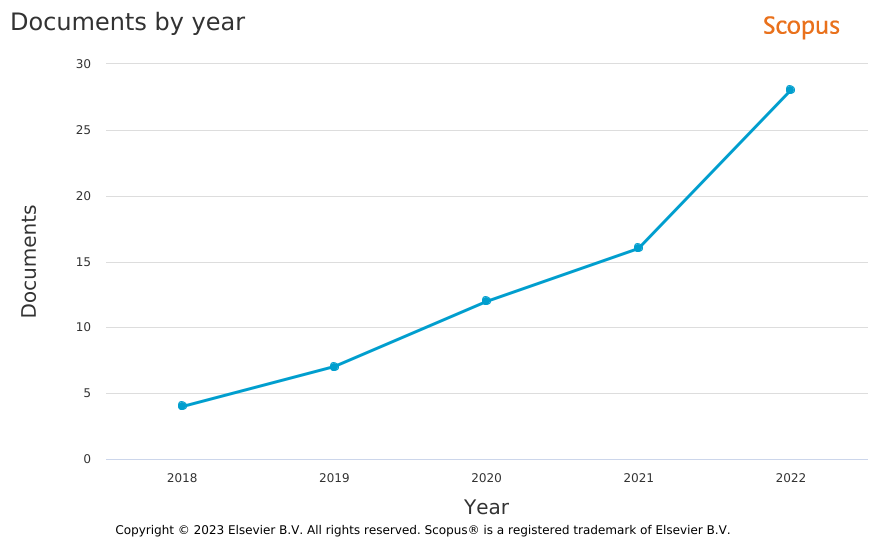
\includegraphics[width=12cm]{../reports/figures/Scopus_Year_ML_RD_AQ.png}
        \label{scopus_year}
        \par
        {\small fonte: Scopus.}
    \end{figure}

    Ao adicionar Cuiabá nas palavras chave da busca, não foi retornado nenhum resultado, isso indica que o trabalho realizado é inédito.

    \begin{table}[ht]
        \centering
        \caption{Publicações no Scopus}
        \label{tabela scopus}
        \begin{tabular}{ccc}
            \hline
            \multicolumn{1}{|c|}{Pesquisa} & \multicolumn{1}{c|}{Período} & \multicolumn{1}{c|}{Total de publicações}\\
            \hline
            "\textit{Machine Learning}" & 2012 - 2022 & 507.100 \\
            "\textit{Machine Learning}" e "Respiratory Diseases" & 2012 - 2022 & 2.338 \\
            "\textit{Machine Learning}" e "Respiratory Diseases"  e "Air Quality" & 2012 - 2022 & 67 \\
            \hline
        \end{tabular}
        \par
        {\small fonte: Scopus (2023)}
    \end{table}

    A \ref*{scopus_country} apresenta a distribuição de trabalhos acadêmicos por países, analisando-a verifica-se que o Brasil tem apenas um trabalho publicado
    na plataforma, o que aponta para uma grande necessidade por novas pesquisas.

    \begin{figure}[ht]
        \centering
        \caption{Distribuição de artigos publicados por país}
        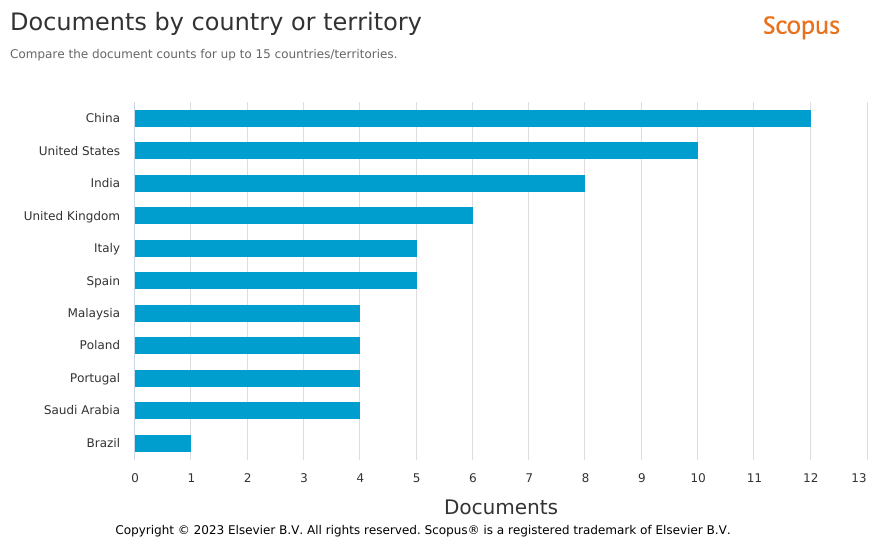
\includegraphics[width=12cm]{../reports/figures/Scopus_Country_ML_RD_AQ.png}
        \label{scopus_country}
        \par
        {\small fonte: Scopus.}
    \end{figure}

    \section{DELIMITAÇÕES DA PESQUISA}
    Ao decorrer do trabalho foram verificadas algumas limitações.
    Os dados utilizados para o treinamento dos modelos de \textit{Machine Learning} e (ANN) possuem 
    colunas com informações sobre a qualidade do ar, temperatura, umidade e internações por doenças respiratórias. Os dados de qualidade
    do ar são estimativas realisadas pelo SISAM para a cidade de Cuiabá-MT, assim considerou-se que todos os habitantes 
    estão submetidos as mesmas condições.

    Ao considerar que todas as pessoas estão influenciadas pelas mesmas condições, desconsidera-se 
    as informações de onde essas pessoas vivem e com o que elas trabalham. Por exemplo, uma pessoa que trabalhe em uma marcenaria
    está sobre condições respiratórias piores do que outras pessoas e essa influência não foi levada em conta nos modelos por não possuir dados.

    Os dados de internações representam apenas as ocorridas nos hospitais da rede pública (SUS). Dessa forma, todas as internações
    por doenças respiratórias ocorridas na rede particular de hospitais não foram contabilizadas. Ainda, as informações das internações por doenças 
    respiratórias são diagnosticadas pelos médicos e inseridas no sistema SIH/SUS, portanto pode haver algum engano ao ser inserida uma informação
    manualmente no sistema.

    \section{ESTRUTURA DO TRABALHO}

    Este trabalho está dividido em 5 partes: 
    
    \begin{itemize}
        \item Introdução
        \item Fundamentação teórica
            \subitem Neste capítulo, será abordado os principais conceitos utilizados para a confecção do trabalho, 
            comentando sobre modelos de aprendizado de máquina, redes neurais artificiais e métricas
            para avaliações dos modelos.
        \item Materiais e métodos
            \subitem Aqui será redigida a descrição do problema, como os dados foram coletados, tratados
            e utilizados nos modelos.
        \item Análise dos resultados obtidos
            \subitem Comparação dos resultados de cada modelo analisando as métricas utilizadas e escolhendo o modelo que obteve os melhores resultados
        \item Conclusão
            \subitem Neste último capítulo será feita uma conclusão do trabalho com propostas de pesquisas futuras.
    \end{itemize}

    \chapter{fundamentação teórica}
    Neste capítulo foi escrita uma descrição resumida das ferramentas, técnicas e conceitos utilizados
    no desenvolvimento do trabalho.
    \section{PYTHON E CIÊNCIA DE DADOS}
    Python é uma linguagem de programação de computadores multiparadigma e de código aberto (\textit{open source}), 
    que de acordo com \cite[]{learning_python} é ótimazada para programar de forma produtiva, ler e entender os códigos
    com facilidade e qualidade de \textit{software}.

    Python é a linguagem mais utilizada do mundo segundo o rank da linguagens de \cite[]{PYPL} ganhando de Java, Java Script e C++. Essa liderança
    explica a extensa comunidade que a linguagem possui, sendo isso uma vantagem para quem utiliza, uma vez que é possível encontrar milhares
    de exemplos de código para uma possível aplicação que alguém precise.
    
    Uma ótima vantagem da linguagem é a íncrivel quantidade de bibliotecas disponibilizadas pela comunidade para as mais variadas aplicações. Isso
    torna o Python uma ótima ferramenta para trabalhar com inteligência artificial, \textit{Machine Learning} e \textit{deep learning}. Algumas das principais
    bibliotecas e \textit{frameworks} utilizadas são Pandas e Numpy para a manipulação de dados, TensorFlow e Scikit Learning para
    a contrução de modelos de \textit{Machine Learning}, como os que serão abordados nos capítulos \ref*{IA} e \ref*{LSTM}.
    
    \section{INTELIGÊNCIA ARTIFICIAL NO CONTEXTO DA SAÚDE}
    \label{IA}
    Inteligência artificial tem sido um assunto amplamente abordado pelas pessoas em vídeos, notícias e filmes. Muitos
    acreditam que as IAs podem ser a solução para todos os problemas existentes na sociedade. No entanto, é importante
    saber o que realmente é inteligência artificial e para o que realmente pode ser usada.

    O professor \cite[]{IA_python} define em seu livro inteligência artificial como sendo uma área de estudo dentro ciências da computação
    que possui o objetivo de fazer com que máquinas aprendam a interpretar e resolver problemas de maneira similar
    ao ser humano. Da mesma forma que um ser humano, aprende ao tentar resolver problemas e obter novas informações, uma inteligência artificial
    deve tomar uma ação a medida em que recebe novas informações e aprende a fim de melhorar sua performance.

    Alguns exemplos de inteligência artificial presente no dia a dia de muitas pessoas são as assistentes virtuais
    como a Alexa da Amazon e a Cortana da Microsoft, outro exemplo são as ferramentas de anúncio na internet que aprendem
    com informações sobre os usuários e enviam anúncios de maior interesse. Mas como as IAs, estam relacionadas 
    com a saúde das pessoas e os serviços de assistência médica?
    
    De acordo com Trishan Panch: 
    \vspace{1.5pt}
            \begin{flushright}
                \begin{minipage}{.724\textwidth}
                    {\SingleSpacing\small
                    A Inteligência Artificial e o aprendizado de máquina têm o potencial de ser o catalisador da transformação
dos sistemas de saúde para melhorar a eficiência e a eficácia, criar margem
para a cobertura universal de saúde e melhorar os resultados. \cite[p.1]{IA_health_systems}
                    }
                \end{minipage}
            \end{flushright}
            \vspace{1.5pt}

    Nos sistemas de saúde existem processos que podem utilizar IAs. Dois exemplos são segundo \cite[]{IA_health_systems}
    o diagnóstico de doenças dos pacientes, realizando uma tarefa de classificação, se está ou não com a doença. O outro processo
    se dá durante o tratamento, envolvendo predição de uma melhora ou piora no quadro do paciente, monitorando os dados vitais. Algumas das
    aplicações existentes foram apresentadas na tabela \ref*{tabela aplicações IA Med}.

    \begin{table}[ht]
        \centering
        \caption{Aplicações de IAs na medicina}
        \label{tabela aplicações IA Med}
        \begin{tabular}{cc}
            \hline
            \multicolumn{1}{|c|}{Diagnóstico} & \multicolumn{1}{c|}{Prognóstico e predição}\\
            \hline
            Analise de imagem: Mamografia & Hospitalização por doença cardíaca\\
            Analise de sinais: Monitoramento intraparto & Risco de acidente cardiovascular\\
            Analise de imagem: identificação da retinopatia diabética& Predição de resultados em câncer colorretal\\
            \hline
        \end{tabular}
        \par
        {\small fonte: Adaptado de \cite[]{IA_health_systems}}
    \end{table}

    Diante disso, é notavel que as IAs podem contribuir para melhorar os serviços de saúde, impactando a vida
    de milhares de pessoas. A seguir serão abordadas algumas técnicas de aprendizado de máquinas utilizadas neste trabalho.

    \subsection{\textit{Decision Trees}}
    
    Árvores de decisão (\textit{Decision Trees}) são algoritmos de \textit{machine learning} muito versáteis, que podem ser utilizados
    tanto para resolver problemas de classificação quanto de regressão.
    Como o próprio nome diz as \textit{Decision Trees} possuem uma estrutura hierarquia em árvore, contendo o nó raiz (\textit{root node}),
    as ramificações, nós de decisão (\textit{decision nodes}) e as folhas (\textit{leaf nodes}). Uma estrutura simples desse algoritmo
    está apresentada na \ref*{estrutura_decision_tree}.

    \begin{figure}[ht]
        \centering
        \caption{Estrutura das árvores de decisão}
        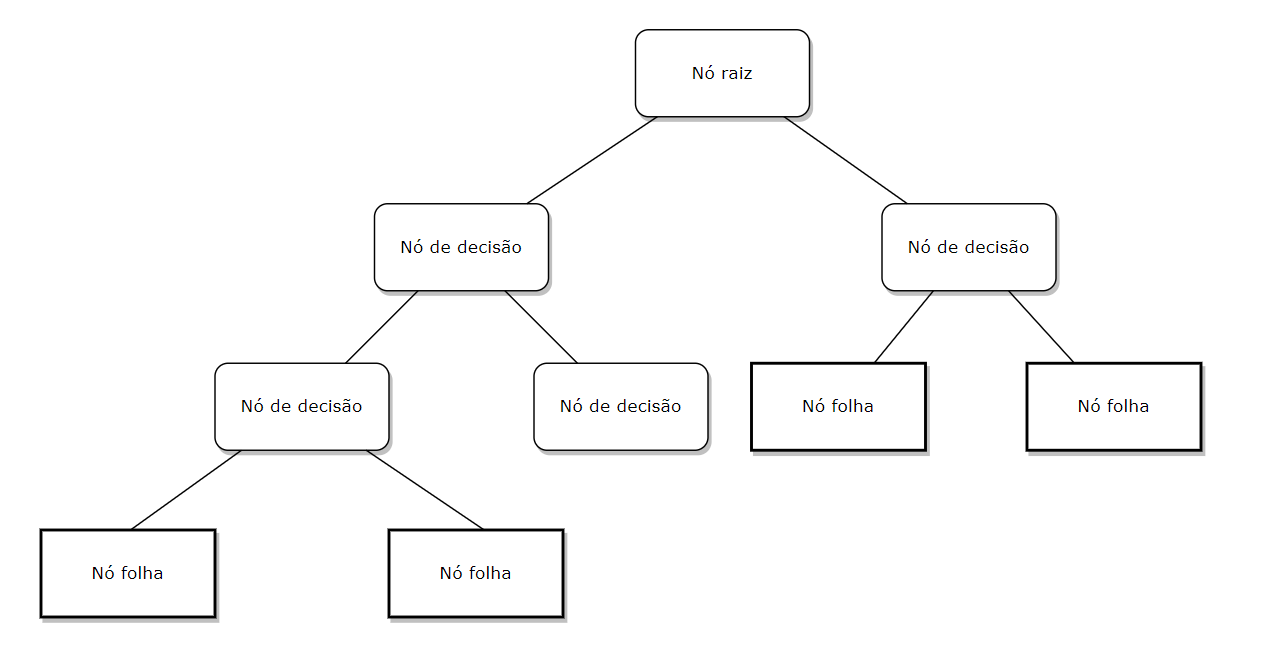
\includegraphics[width=13cm]{../reports/figures/decision_tree_exemple.png}
        \label{estrutura_decision_tree}
        \par
        {\small fonte: Produção do próprio autor.}
    \end{figure}

    O modelo de \textit{Decision Tree} utilizado nesse trabalho realizou uma tarefa de regressão, ou seja, uma \textit{Regresion Tree}, nessa variação 
    todos os nós da árvore possuem valores numéricos. Imaginando um conjunto de pontos (x, y), o primeiro passo para montar a árvore é obter o 
    nó raiz, sendo encontrado ao calcular iterativamente para o valor médio entre dois x adjacentes o erro quadrático médio (MSE) com a média
    dos valores de y a esquerda do ponto médio e a média dos valores de y a direita do ponto médio. O valor médio que obtiver o menor MSE
    será o nó raiz da árvore.

    Para finalizar todo o processo de construção o processo é repetido para o lado esquerdo do nó raiz e para o lado direito até que não sobrem mais
    valores possíveis para as folhas.

    \subsection{\textit{Random Forest}}
    \label{rf}

    O \textit{random forest} (floresta aleatória) é um algoritmo de machine learning do tipo aprendizagem 
    supervisionada que pode ser utilizado tanto para resolver problemas de classificação quanto de regressão. 
    O RF foi desenvolvido, com o intuito de resolver algumas desvantagens observadas nos modelos de \textit{decision tree}.
    
    O conceito de florestas está na construção da \textit{random forest}, em que é construída realizando um agrupamento 
    de \textit{decision tree} durante o treinamento, chamado de método \textit{ensemble}, ou seja, reúne a predição 
    dos múltiplos algoritmos pela média, resultando em uma predição mais acurada do que apenas uma \textit{decision tree}. 
    Conforme apresentado na \ref*{estrutura_random_florest}:

    \begin{figure}[ht]
        \centering
        \caption{Estrutura da \textit{random florest}}
        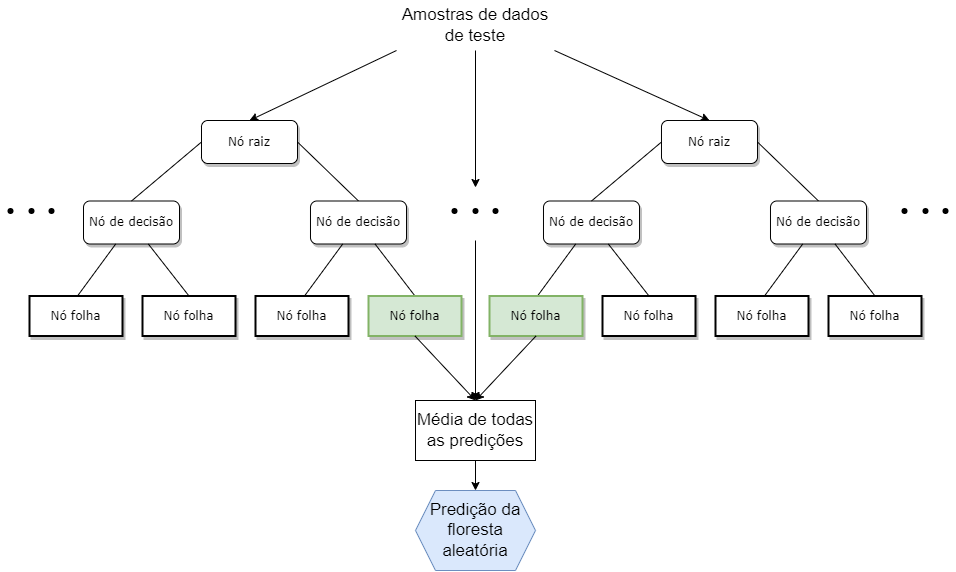
\includegraphics[width=12cm]{../reports/figures/random_forest.png}
        \label{estrutura_random_florest}
        \par
        {\small fonte: Produção do próprio autor.}
    \end{figure}
    
    O funcionamento do algoritmo ocorre da seguinte forma, primeiramente, deve-se escolher o número de árvores de decisão, 
    então selecionam-se os dados de forma aleatória podendo haver repetições, repetindo o processo para o número de 
    \textit{decison tree} escolhido. Após isso, as árvores são construídas a partir dos dados aleatórios selecionados para cada uma,
    por isso nomeia-se floresta aleatória.
    \subsection{\textit{Cross Validation}}
    Existem diferentes modelos de \textit{machine learning} disponíveis que podem ser empregados na resolução de problemas, 
    e como consequência dessas possibilidades aparecem algumas dúvidas:

    \begin{itemize}
        \item Qual modelo é melhor?
        \item Qual modelo terá o melhor desempenho?
        \item Qual será o mais estável ao receber \textit{inputs} inéditos?
    \end{itemize}

    Antes de realizar o treino e o teste do modelo é necessário preparar o conjunto de dados em que filtrar ruídos e tratar valores
    nulos são exemplos de passos que podem ser aplicados. Após essa etapa, o conjunto de dados é randomizado
    e divindo-o em teste e treino, de acordo com \cite[]{hands_on_ml} é comum dividir o conjunto de dados em 80\% treino
    e 20\% teste, no entanto em casos que a quantidade de dados é massiva, diminuir o percentual dos dados de teste pode ser
    uma boa prática.

    Ao realizar esses passos será obtido um conjunto de acordo com a \ref*{exemplo_treino_teste}.

    \begin{figure}[ht]
        \centering
        \caption{Exemplo de um conjunto de treino e teste}
        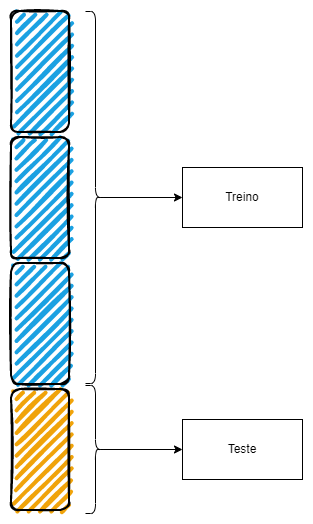
\includegraphics[width=5cm]{../reports/figures/treino_teste_exemplo.png}
        \label{exemplo_treino_teste}
        \par
        {\small fonte: Produção do próprio autor.}
    \end{figure}

    Um possível problema dessa abordagem é a utilização de apenas a última parte do \textit{dataset} para o treino, isso porque,
    mesmo que apresente um erro de generalização pequeno, ao colocar o modelo em produção dados completamente inéditos e diferentes
    do conjunto de teste podem aparecer, mostrando que o modelo não generaliza tão bem quanto o esperado.

    Uma solução para esse problema é a validação cruzada (\textit{cross validation}), uma técnica muito empregada para avaliar o desempenho de
    modelos com relação a todo o conjunto de dados, a fim de verificar qual modelo obtem a melhor generalização.

    A validação cruzada consiste em particionar o conjunto de dados em partes iguais, sendo a quantidade de partes escolhidas
    arbitrariamente. A \ref*{exemplo_cross_val} exemplifica uma \textit{4-fold cross validation}, ou seja, o conjunto de dados
    dividido em 4 partes. Os modelos são então treinados 4 vezes, variando a ordem das partições de treino e teste, ao final
    faz-se a média do erro de generalização e verifica qual modelo mostrou ter o melhor desempenho em todo o conjunto de dados.
    Esse será o melhor a ser utilizado.

    \begin{figure}[ht]
        \centering
        \caption{Exemplo do funcionamento da validação cruzada}
        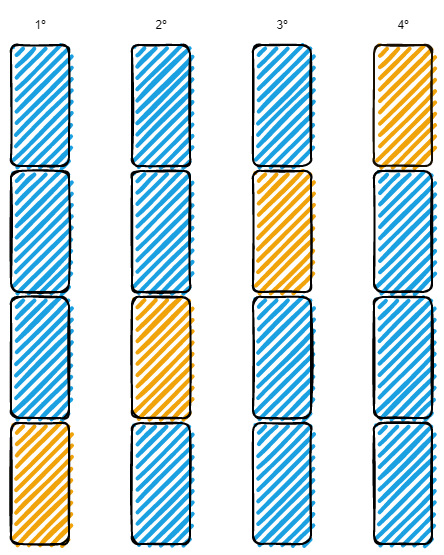
\includegraphics[width=10cm]{../reports/figures/cross_validation_example.png}
        \label{exemplo_cross_val}
        \par
        {\small fonte: Produção do próprio autor.}
    \end{figure}
    
    \section{PREVISÃO DE SÉRIES TEMPORAIS NO CONTEXTO DA SAÚDE}
    Uma série temporal, ou série histórica, é definida segundo \cite[]{series_temporais}
    como uma sequência de dados obtidos em intervalos regulares durante um determinado período.
    A série pode ser obtida tanto ao realizar medições por sensores, por exemplo, temperatura, pressão, 
    tanto por contagens, por exemplo, o número de internações mensais por doenças respiratórias.

    A previsão de séries temporais é utilizada no âmbito dos sistemas de saúde em diferentes contextos, como 
    previsão de epidemias de doenças antigas e novas e previsão das demandas no sistema de sáude, por internações, atendimentos e cirurgias.
    Conforme \cite[]{forcasting_health} os serviços de saúde geralmente estão mal informados 
    e com recursos insuficientes para se adaptar a períodos como alta demanda, por isso, utilizar uma abordagem
    de séries temporais, pode ser útil para promover melhores informações e ajudar em tomada de 
    decisões mais eficientes por médicos e administradores do sistema de serviço de saúde.

    \subsection{\textit{Long Short Term Memories}}
    \label{LSTM}
    As \textit{Long Short Term Memories} são um tipo específico de rede neural recorrente (RNN) que tem como objetivo
    resolver o problema do \textit{explode/vanishing gradient} da RNN original. Para isso elas utilizam dois caminhos
    diferentes para realizar uma predição, o caminho de memória curta \textit{short term} e o caminho de memória longa
    \textit{long term}.

    As LSTMs possuem uma unidade mais complicada do que as RNNs tradicionais, conforme apresentado na \ref*{lstm_unit}.
    \begin{figure}[ht]
        \centering
        \caption{Exemplo de uma unidade LSTM}
        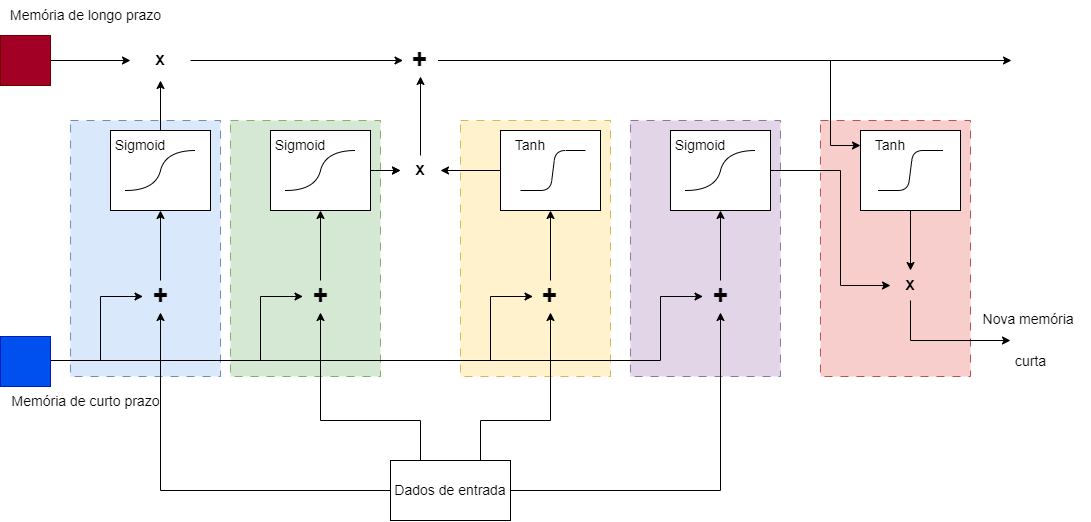
\includegraphics[width=12cm]{../reports/figures/LSTM_unit.png}
        \label{lstm_unit}
        \par
        {\small fonte: Adaptado de \cite[]{statquest}.}
    \end{figure}

    As memórias de curto e longo prazo podem ser iniciadas com um valor arbitrário, geralmente sendo 0. Então, analisando
    de forma sequencial, o primeiro bloco (azul) da unidade LSTM, é responsável por determinar quanto da memória de longo prazo será lembrada,
    isso porque a saída desse bloco é uma função sigmoidal, portanto quando o dado de entrada soma-se a memória de curto prazo, são aplicados
    na função sigmoidal resultando em um valor entre 0 e 1, esse primeiro bloco é chamado de \textit{forget gate}.
    A próxima etapa de processamento da unidade são o conjunto de blocos verde e amarelo (\textit{input gate}), sendo a sua função calcular 
    quanto um valor a ser somado na memória de longo prazo, o bloco verde gera a porcentagem a ser somada e o bloco amarelo
    uma memória em potencial.
    A última etapa da LSTM é o \textit{output gate} que relaciona a memória de curto prazo a entrada e a memória de longo prazo
    para produzir uma nova memória de curto prazo. A saída da LSTM \textit{unit} pode ser utilizada tanto para a predição do modelo ou para entrada para a próxima unidade
    em uma rede neural artificial LSTM.

    Resumindo, de acordo com \cite[]{hands_on_ml} as unidades LSTM aprendem a reconhecer entradas importantes da série temporal, 
    armazenando-as na memória de longo prazo, para prezerva-lá por um certo tempo e assim, reutiliza-lá sempre que necessário. 
    Essa estrutura robusta são o motivo da LSTM obter performances tão boas em detectar padrão de longo prazo 
    em séries temporais, textos longos e gravações de áudio.


    \section{MÉTRICAS PARA AVALIAR OS MODELOS DE REGRESSÃO}
    Durante a estimativa dos parâmetros de um modelo de regressão, é necessária a utilização de métricas
    para a validação da sua performance. Nesse contexto, as métricas mais utilizadas são as relacionadas
    ao erro entre a predição e o valor esperado, sendo algumas métricas, erro médio absoluto (MAE), percentual do erro médio absoluto (MAPE), 
    erro quadárico médio (MSE) e raíz do erro quadárico médio (RMSE).

    \subsection{Erro quadrático médio}
    O MSE é calculado pela equação \ref*{mse}: 

    \begin{equation}
        \label{mse}
        \sum_{i=1}^{D}(y_i-yhat_i)^2
    \end{equation}

    Analisando a equação, percebe-se que como o erro está elevado ao quadrado nunca haverá um valor negativo e
    um outro efeito dessa métrica é punir o modelo quanto maior for o erro, uma vez que, um número grande elevado ao quadrado
    será um número ainda maior.
    
    \subsection{Raiz do erro quadrático médio}
    O RMSE é calculado pela equação \ref*{rmse}: 

    \begin{equation}
        \label{rmse}
        \sqrt{\sum_{i=1}^{D}(y_i-yhat_i)^2}
    \end{equation}
    
    Essa métrica é mais empregada para analisar a performance do modelo e mostrar os resultados, enquanto o
    MSE é utilizado como \textit{loss function}. Outro ponto importante é a unidade do erro que é a mesma do valor de saída.
    \subsection{Erro médio absoluto}
    O MAE é calculado pela equação \ref*{mae}: 

    \begin{equation}
        \label{mae}
        \sum_{i=1}^{D}|x_i-y_i|
    \end{equation}

    Diferentemente do MSE, essa métrica não intensifica o erro, quanto maior for, mas varia linearmente com o aumento
    ou diminuição do erro.
    
    \chapter{materiais e métodos}
    Nesse capítulo será realizada toda a descrição do problema, desde a escolha da cidade de Cuiabá,
    as queimadas ocorridas, até os principais poluentes analisados.

    \section{DESCRIÇÃO DO PROBLEMA}
    Cuiabá é a capital do estado do Mato Grosso, localizada na região centro-oeste do Brasil e reconhecida
    por ser o principal polo industrial, comercial e de serviços do seu estado. A Tabela \ref*{tabela cuiaba} apresenta algumas informações
    da cidade:

    \begin{table}[ht]
        \centering
        \caption{Informações da cidade de Cuiabá}
        \label{tabela cuiaba}
        \begin{tabular}{cc}
            \hline
            \multicolumn{1}{|c|}{Métricas} & \multicolumn{1}{c|}{Valores}\\
            \hline
            Área territorial & 5.077,181 km² [2021]\\
            População estimada & 623.614 pessoas [2021]\\
            Densidade demográfica & 157,66 hab/km² [2010]\\
            Mortalidade infantil & 12,92 óbitos por mil nascidos vivos [2020]\\
            PIB per capita & 42.918,31 R\$ [2020]\\
            \hline
        \end{tabular}
        \par
        {\small fonte: Adaptado de \cite[]{ibge}}
    \end{table}

    Segundo dados do \cite[]{ibge_mais} 80,2\% dos domicílios possuem esgotamento
    sanitário adequado, apenas 39,6\% dos domicílios urbanos tem arborização e
    34,3\% com urbanização adequada.

    Ainda, de acordo com uma notícia de \cite[]{queimadas_cuiaba} o índice de material
    particulado durante queimadas no ano de 2017 oscilou entre 100 e 140 µg/m³, valor
    muito maior do que o mínimo considerado tolerável pelo ser humano de 25µg/m³. Esses valores
    altos observados contribuem para o surgimento de problemas respiratórios graves, como o
    broncoespasmo, que causa o estreitamento das vias respiratórias e, portanto, dificuldade de
    respirar. Além disso, essa poluição causa irritação das vias aéreas, tornando-as mais
    sucetíveis a vírus e bactérias levando muitas pessoas a ter infecções graves como a pneumonia. 
    Sendo outros problemas comuns as crises de asma, bronquites,
    crises alérgicas, rinites, sinusites e irritação nos olhos.

    Diante desse contexto, tornou-se evidente a importância do presente tema desse trabalho. Ao analisar
    como diferentes modelos de aprendizado de máquina e uma rede neural artificial performam com os dados
    utilizados e sua capacidade de predição de novas internações por doenças respiratórias, pode ser uma
    importante ferramenta para, principalmente, ajudar a salvar mais vidas, gerenciar recursos e
    melhorar a qualidade de vida da população.

    Os principais poluentes utilizados nos treinamentos dos modelos foram o ozônio em partes por bilhão e
    o material particulado de 2,5 micrômetros (µg/m³), além dessas \textit{features}, o banco de
    dados, também conta com dióxido de enxofe ($SO_2$ [µg/m³]) e monóxido de carbono ($CO$ [ppb]). As informações
    climáticas e ambientais são a temperatura média diária [\textdegree C], umidade relatival percentual, 
     precipitação pluviométrica diária [mm] e os focos de queimadas na cidade. Por fim, o banco contém 
    a quantidade diária de internações ocorridas por doênças e complicações respiratórias nos hospitais públicos
    de Cuiabá. 

    \section{OBTENÇÃO DOS DADOS}
    
    Os dados utilizados para o projeto foram retirados de dois bancos de dados governamentais: O 
    Sistema de Informações Ambientais Integrado a Saúde (SISAM) e o Sistema de informações hospitalares do SUS (SIHSUS).

    O site do SISAM disponibiliza na aba Dados/Downloads uma interface para realizar a filtragem dos dados desejados e 
    fazer a requisição de download, conforme apresentado na \ref*{int_sisam}:

    \begin{figure}[ht]
        \centering
        \caption{Interface do SISAM}
        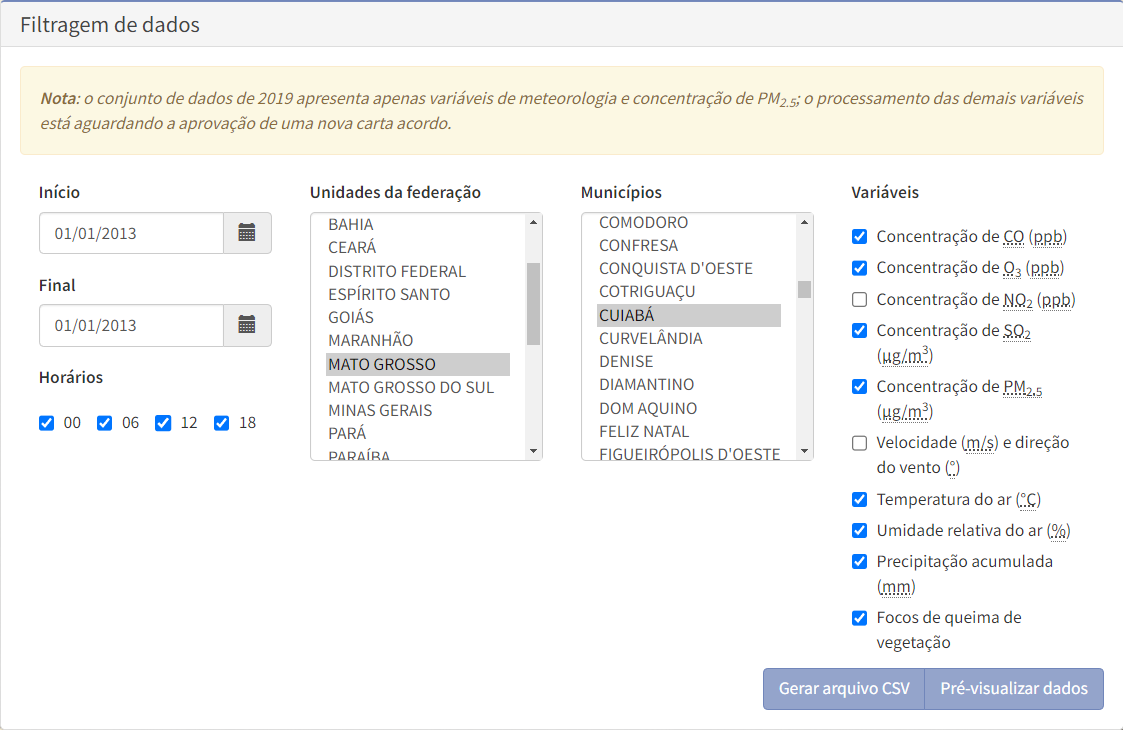
\includegraphics[width=12cm]{../reports/figures/interface_SISAM.png}
        \label{int_sisam}
        \par
        {\small fonte: SISAM.}
    \end{figure}

    No sistema é possível escolher um período de até 1 ano, o estado e a cidade, as variáveis 
    meteorológicas e poluentes. Então, clica-se em "gerar arquivo csv" para realizar o download de todos os
    dados selecionados.

    O projeto utilizou 6 anos de dados que englobou os períodos de primeiro de Janeiro de 2013 
    até 31 de dezembro de 2018, dessa forma fez-se 6 vezes o download dos dados para cada ano até 2018.
    Foi necessário juntar todos os arquivos em um único, isso foi feito por meio da biblioteca Pandas do Python.

    Para cada dia haviam 4 horários de medições, por isso, o tratamento escolhido foi 
    calcular a média diária para todas as colunas dos dados. 
    A \ref*{sisam_not_filtered}, apresenta os dados antes do tratamento com 8.764 linhas 
    e possuindo valores nulos nas colunas precipitacao\_mmdia e focos\_queimada.
    
    \begin{figure}[ht]
        \centering
        \caption{Dados com 4 medições diárias}
        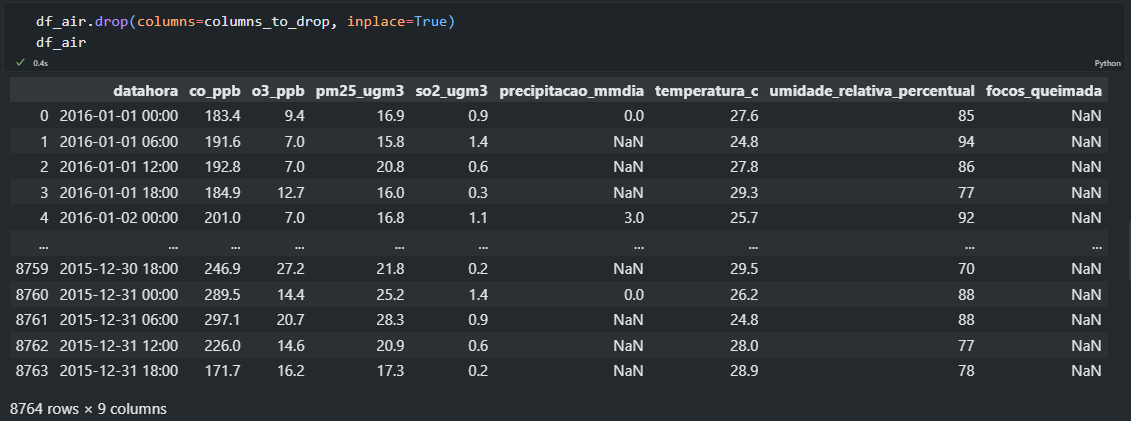
\includegraphics[width=12cm]{../reports/figures/sisam_not_filtered.png}
        \label{sisam_not_filtered}
        \par
        {\small fonte: Produção do próprio autor.}
    \end{figure}

    A \ref*{sisam_filtered} apresenta os dados agrupados por dia, sendo cada valor diário a média das 4 medições diárias, os dados
    nulos da coluna de focos de queimadas foram substituidos por 0. Dessa forma, o conjunto de dados climáticos e de poluentes ficou
    com 2.191 linhas que são exatamente 6 anos.

    \begin{figure}[ht]
        \centering
        \caption{Dados filtrados e tratados}
        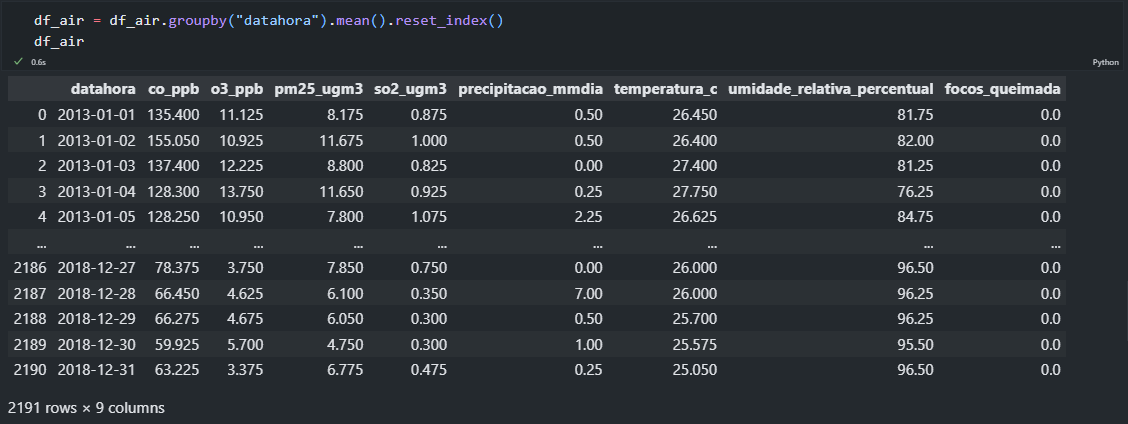
\includegraphics[width=12cm]{../reports/figures/filter_sisam.png}
        \label{sisam_filtered}
        \par
        {\small fonte: Produção do próprio autor.}
    \end{figure}

    A obtenção dos dados de internações por doenças respiratórias foi através do sistema de transferência
    de arquivos do site Datasus. No site é necessário selecionar a fonte: Sistema de informações hospitalares do SUS (SIHSUS),
    modalidade: Dados, tipo de arquivo: RD - AIH Reduzida, o período desejado, nesse caso 2013 até 2018, quais meses do ano, sendo
    para esse projeto todos os meses e o estado: MT (Mato Grosso), conforme apresentado na \ref*{interface_datasus}.

    \begin{figure}[ht]
        \centering
        \caption{Interface de coleta de dados do Datasus}
        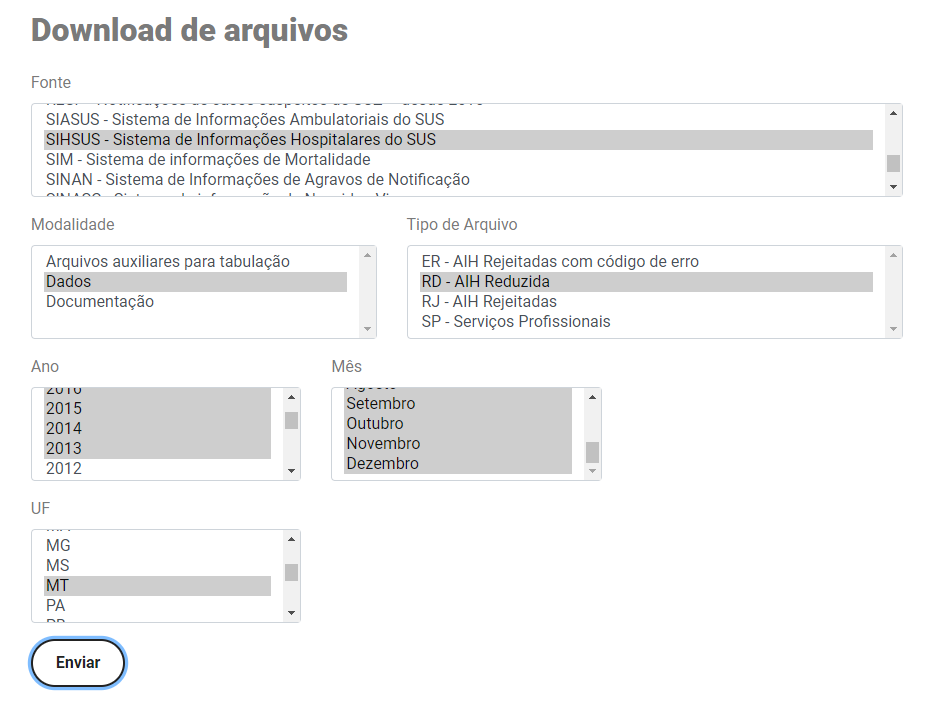
\includegraphics[width=12cm]{../reports/figures/interface_datasus.png}
        \label{interface_datasus}
        \par
        {\small fonte: Datasus.}
    \end{figure}

    Após selecionar o botão enviar, uma lista de arquivos aparece para serem baixados e conforme a descrição acima foram
    retornados 72 arquivos. Os 6 primeiros aparecem na \ref*{arquivos_datasus}.

    \begin{figure}[ht]
        \centering
        \caption{Arquivos para \textit{download} do Datasus.}
        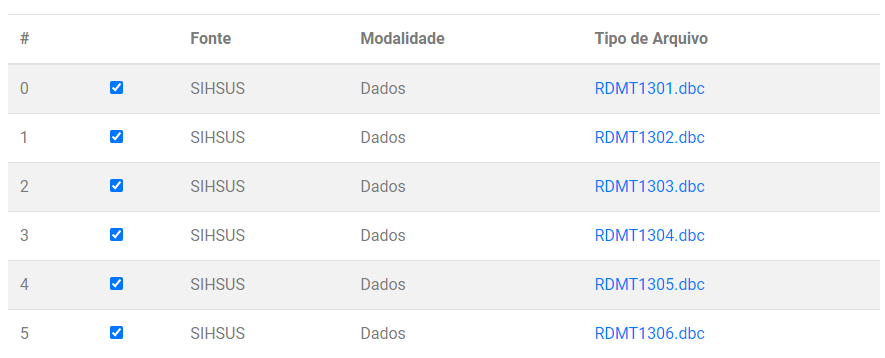
\includegraphics[width=12cm]{../reports/figures/arquivos_datasus.png}
        \label{arquivos_datasus}
        \par
        {\small fonte: Datasus.}
    \end{figure}

    Os arquivos estão em formato .dbc, esse formato impossibilita manipular os arquivos pela ferramenta Pandas, por isso, 
    foi utilizado o \textit{software} TABWIN disponibilizado pelo Datasus. Nesse programa os arquivos são primeiramente
    expandidos para .dbf, após isso é possível converter um arquivo por vez para .csv, possibilitando a manipulação
    em código. Observa-se os processos de conversão nas \ref*{dbf_datasus} e \ref*{csv_datasus}.

    \begin{figure}[ht]
        \centering
        \caption{Conversão dos arquivos em .dbf.}
        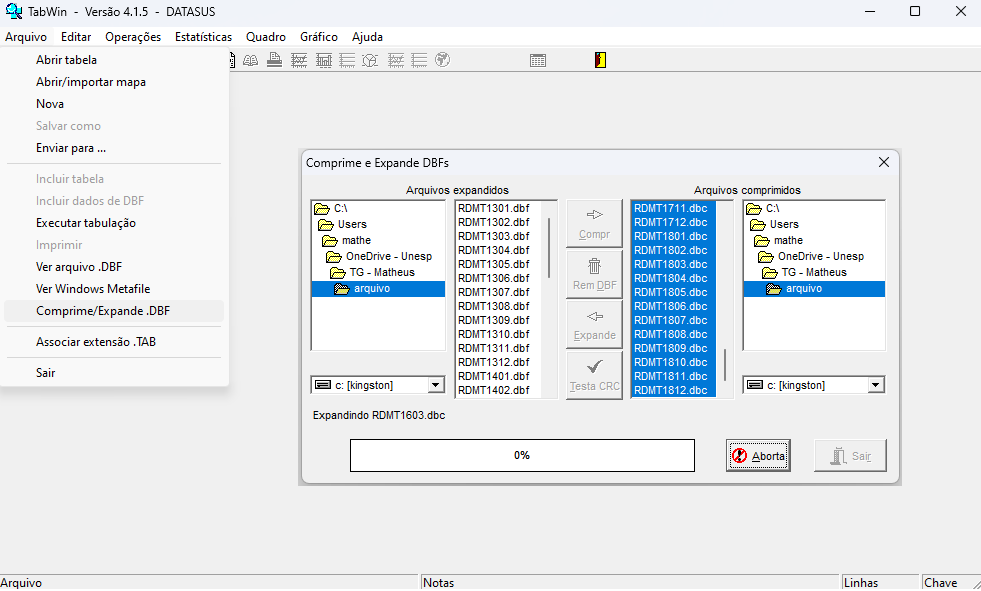
\includegraphics[width=12cm]{../reports/figures/tabwin_process.png}
        \label{dbf_datasus}
        \par
        {\small fonte: Produção do próprio autor.}
    \end{figure}

    \begin{figure}[ht]
        \centering
        \caption{Conversão dos arquivos em .csv.}
        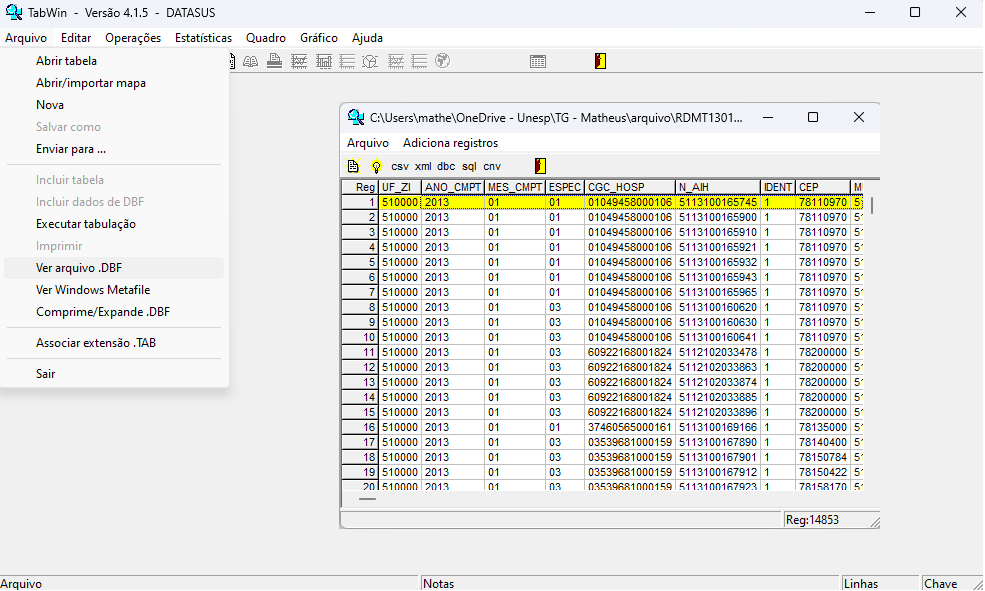
\includegraphics[width=12cm]{../reports/figures/csv.png}
        \label{csv_datasus}
        \par
        {\small fonte: Produção do próprio autor.}
    \end{figure}

    Agora, com os arquivos do Datasus em extensão csv realizou-se a filtragem das colunas de interesse, sendo as colunas, a data e o
    diagnóstico da internação filtrando para a cidade de Cuiabá. Fez-se a soma das internações por problemas
    respirátórios para cada dia. O resultado obtido pode ser observado na \ref*{resp_dataset}.

    \begin{figure}[ht]
        \centering
        \caption{Tratamento final dos dados de doenças respiratórias.}
        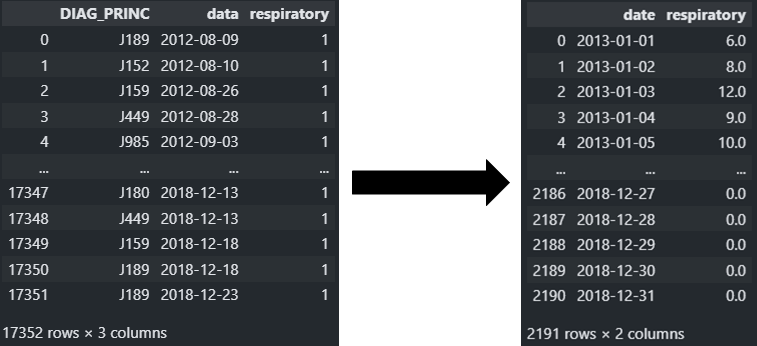
\includegraphics[width=12cm]{../reports/figures/filter_csv_resp.png}
        \label{resp_dataset}
        \par
        {\small fonte: Produção do próprio autor.}
    \end{figure}

    Conforme apresentado na \ref*{resp_dataset} os diagnóticos de doenças possuem um código, para selecionar apenas as doenças
    respiratórias, verificou-se o índice de Classificação Internacional de Doenças (CID-10), no índice, observa-se que a 
    seção "J" reune os códigos das doenças respiratórias, dessa dorma fez-se a seleção apenas dos códigos que começavam com a letra J
    na base do Datasus.

    Para finalizar a obtenção dos dados foi realizada a junção das duas tabelas: dados do SISAM e diagnóstico das internações. 
    A tabela resultante está apresentada na \ref*{tabela_completa}.

    \begin{figure}[ht]
        \centering
        \caption{Tabela com todas as \textit{features} necessárias para os treinamentos dos modelos}
        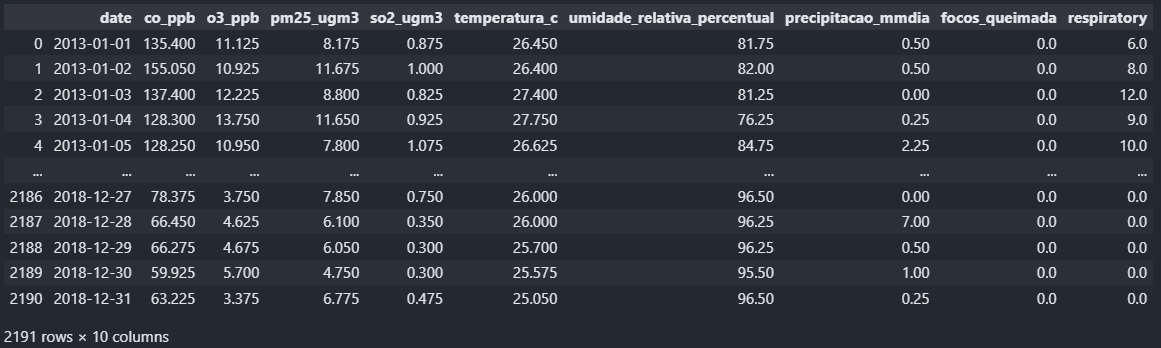
\includegraphics[width=12cm]{../reports/figures/df_complete.png}
        \label{tabela_completa}
        \par
        {\small fonte: Produção do próprio autor.}
    \end{figure}

    \section{MODELAGEM DO PROBLEMA}

    A modelagem do problema foi dividida da em duas abordagens distintas, isso porque, como os dados 
    são uma série temporal e o problema foi classificado como sendo de regressão, optou-se na primeira abordagem por
    utilizar os modelos de \textit{machine learning} sem se importar com a característica temporal dos dados. A segunda
    abordagem, diferentemente da primeira, foi modelar uma rede LSTM tratando como importante a característica temporal
    dos dados para encontrar padrões na série e predizer o número de pacientes internados por doenças respiratórias.

    Em todos os modelos apenas 3 \textit{features} foram utilizadas nos treinamentos, sendo elas:
    o3\_ppb, pm25\_ugm3, temperatura\_c, umidade\_relativa\_percentual. A variação da quantidade de variáveis
    de entrada pode ser realizada em trabalhos futuros.

    O objetivo principal é avaliar quais dos modelos desempenhará melhor e comparar as abordagens.

    \subsection{Primeira abordagem}
    Antes de iniciar o treinamento dos modelos de \textit{machine learning} é necessário fazer um tratamento dos
    dados a fim de maximizar o desempenho dos modelos.

    O primeiro passo foi criar uma coluna apenas com o valor de cada ano, após isso, fez-se a divisão
    dos dados em 80\% para treino e 20\% para teste utilizando a função \textit{"train\_test\_split"} da biblioteca
    \textit{"sklearn"}, conforme apresentado na \ref*{estratificado} configurou-se o parâmetro \textit{"stratify"} para estratificar os dados
    pela coluna com o valor dos anos. Isso para que o conjunto de treino e teste mesmo aleatorizados tenham a mesma
    quantidade de valores aleatórios por ano. Assim, evitar que um determinado ano por ter mais dados após realizar o \textit{split}
    tenha mais influência no modelo do que os outros anos.

    \begin{figure}[ht]
        \centering
        \caption{Comparação entre estratificar o \textit{dataset} por ano e apenas randomizar}
        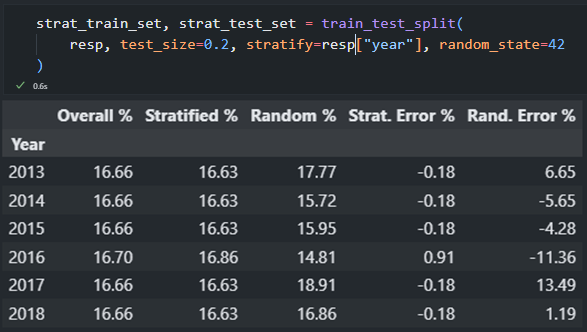
\includegraphics[width=12cm]{../reports/figures/estratificar.png}
        \label{estratificado}
        \par
        {\small fonte: Produção do próprio autor.}
    \end{figure}

    Uma análise de correlação linear entre as \textit{features} e a variável de predição foi realizada a fim de identificar
    quais \textit{features} tinha uma capacidade maior de informar uma tendencia na variável de saída. Conforme apresentado na Tabela
    \ref*{corr_table} nenhuma das variáveis de entrada apresentou correlação linear, isso não significa que elas não servem para 
    predizer o número de internações por doenças respiratórias, mas sim que a saída não varia linearmente com algumas
    das entradas.

    \begin{table}[ht]
        \centering
        \caption{Correlação linear entre as \textit{features} e a variável de saída}
        \label{corr_table}
        \begin{tabular}{cc}
            \hline
            \multicolumn{1}{|c|}{\textit{features}} & \multicolumn{1}{c|}{correlação}\\
            \hline
            so2\_ugm3 & 0.029319\\
            o3\_ppb & -0.009726\\
            temperatura\_c & -0.028572\\
            co\_ppb & -0.047439\\
            precipitacao\_mmdia & -0.064309\\
            pm25\_ugm3 & -0.091198\\
            umidade\_relativa\_percentual & -0.171462\\
            \hline
        \end{tabular}
        \par
        {\small fonte: Produção do próprio autor.}
    \end{table}

    A última etapa antes do treinamento é a construção de uma \textit{pipeline} que tem a função de executar funções
    de transformações do \textit{dataframe} de treino antes de ser aplicado no modelo. Foi feita a construção de uma 
    \textit{pipeline} simples com o \textit{"StandardScaler"} que subtrai do valor de cada \textit{feature} pela média e divide pelo desvio padrão
    , esse processo é conhecido como normalização e sendo um requerimento comum para os modelos de aprendizado de máquina.

    \subsubsection{Modelo de regressão linear}

    O modelo de regressão linear foi escolhido como base de comparação por ser um dos modelos mais simples e assim
    comparar com os estimadores mais sofisticados.

    A API do \textit{sklearn} é simples e intuitiva, a \ref*{lin_reg} apresenta o código utilizado para a construção do modelo:

    \begin{figure}[ht]
        \centering
        \caption{Construção do modelo de regressão linear}
        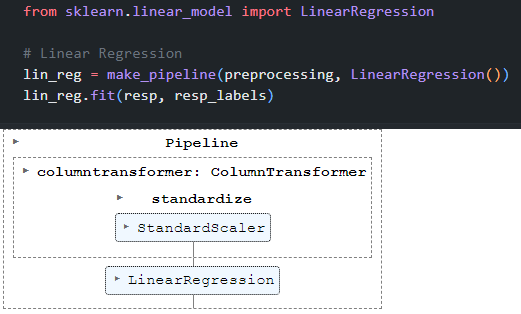
\includegraphics[width=12cm]{../reports/figures/linear_reg.png}
        \label{lin_reg}
        \par
        {\small fonte: Produção do próprio autor.}
    \end{figure}

    \subsubsection{\textit{Decision Tree}}
    
    O \textit{Decison Tree} foi utilizado por ser realmente mais robusto que a regressão linear e de acordo com \cite[]{hands_on_ml} é capaz de encontrar
    complexas relações de correlações não lineares.

    O código para a construção da árvore de decisão está na \ref*{tree_reg}:

    \begin{figure}[ht]
        \centering
        \caption{Construção do modelo de árvore de decisão}
        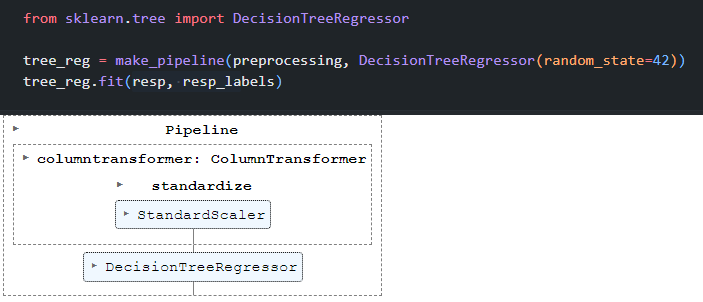
\includegraphics[width=12cm]{../reports/figures/decision_tree_model.png}
        \label{tree_reg}
        \par
        {\small fonte: Produção do próprio autor.}
    \end{figure}

    \subsubsection{\textit{Random Forest}}

    O modelo de floresta aleatória como descrito no capítulo \ref*{rf} tem um aumento de robustez e melhoria em alguns pontos
    relacionados a uma \textit{Decision Tree} simples, o \textit{Random Forest} faz um conjunto de unidades de árvores de decisão
    diminuindo a possibilidade de \textit{overfitting}.

    De maneira semelhante ao código anterior, a \ref*{rf_reg} apresenta a construção do modelo:

    \begin{figure}[ht]
        \centering
        \caption{Construção do modelo de floresta aleatória}
        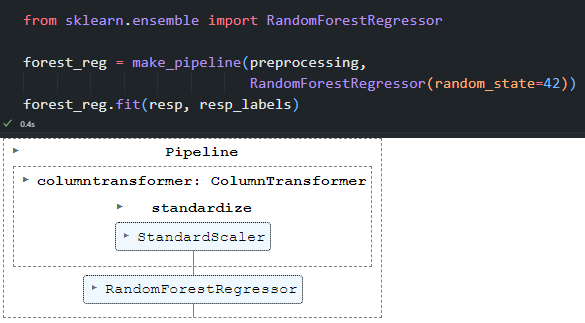
\includegraphics[width=12cm]{../reports/figures/rf_model.png}
        \label{rf_reg}
        \par
        {\small fonte: Produção do próprio autor.}
    \end{figure}

    \subsection{Segunda abordagem}

    A segunda abordagem baseia-se na utilização dos dados arranjados como uma série temporal e para
    isso decidiu-se modelar uma RNN do tipo LSTM. As redes LSTM consomem dados em formato de série temporal, portanto
    nessa nova abordagem necessitou-se realizar novamente o tratamente da base de dados para essa aplicação.

    Os dados foram ordenados por ordem cronológica e então fez-se a normalização utilizando a ferramenta \textit{"MinMaxScaler"} do
    \textit{framework} \textit{"sklearn"}. O normalizador utilizado foi configurado para transformar os dados entre 0 e 1 
    para que todos os dados tenham a mesma ordem de grandeza ajudando no desempenho da RNN.

    Após a normalização realizou-se a transformação dos dados para se adequar a um problema de aprendizado
    supervisionado em séries históricas, dessa forma é possível considerar um \textit{lag} da quantidade de dias
    desejados. Isso significa que condições climáticas e de qualidade do ar não provocam, necessariamente, uma complicação
    respiratória a uma pessoa no mesmo dia, mas pode levar a pessoa a se sentir mal e procurar ajuda médica
    dias depois. Considerando um \textit{lag} de 3 dias, observa-se a transformação dos dados na Tabela \ref*{tab:series_to_supervised}.


    \afterpage{
        \clearpage
        \begin{landscape}
            \centering
            \begin{longtable}{cccccccccccc}
\caption{Transformação dos dados para aprendizado supervisionado (lag=3 dias)}
\label{tab:series_to_supervised}\\
\toprule
 var1(t-3) &  var2(t-3) &  var3(t-3) &  var1(t-2) &  var2(t-2) &  var3(t-2) &  var1(t-1) &  var2(t-1) &  var3(t-1) &  var1(t) &  var2(t) &  var3(t) \\
\midrule
\endfirsthead
\caption[]{Transformação dos dados para aprendizado supervisionado (lag=3 dias)} \\
\toprule
 var1(t-3) &  var2(t-3) &  var3(t-3) &  var1(t-2) &  var2(t-2) &  var3(t-2) &  var1(t-1) &  var2(t-1) &  var3(t-1) &  var1(t) &  var2(t) &  var3(t) \\
\midrule
\endhead
\midrule
\multicolumn{12}{r}{{Continued on next page}} \\
\midrule
\endfoot

\bottomrule
\endlastfoot
  0.025462 &   0.746212 &   0.214286 &   0.037227 &   0.750000 &   0.285714 &   0.027563 &   0.738636 &   0.428571 & 0.037143 & 0.662879 & 0.321429 \\
  0.037227 &   0.750000 &   0.285714 &   0.027563 &   0.738636 &   0.428571 &   0.037143 &   0.662879 &   0.321429 & 0.024202 & 0.791667 & 0.357143 \\
  0.027563 &   0.738636 &   0.428571 &   0.037143 &   0.662879 &   0.321429 &   0.024202 &   0.791667 &   0.357143 & 0.017563 & 0.772727 & 0.142857 \\
  0.037143 &   0.662879 &   0.321429 &   0.024202 &   0.791667 &   0.357143 &   0.017563 &   0.772727 &   0.142857 & 0.018655 & 0.791667 & 0.214286 \\
  0.024202 &   0.791667 &   0.357143 &   0.017563 &   0.772727 &   0.142857 &   0.018655 &   0.791667 &   0.214286 & 0.025210 & 0.803030 & 0.250000 \\
  0.017563 &   0.772727 &   0.142857 &   0.018655 &   0.791667 &   0.214286 &   0.025210 &   0.803030 &   0.250000 & 0.036134 & 0.833333 & 0.500000 \\
  0.018655 &   0.791667 &   0.214286 &   0.025210 &   0.803030 &   0.250000 &   0.036134 &   0.833333 &   0.500000 & 0.035630 & 0.837121 & 0.142857 \\
  0.025210 &   0.803030 &   0.250000 &   0.036134 &   0.833333 &   0.500000 &   0.035630 &   0.837121 &   0.142857 & 0.032269 & 0.750000 & 0.142857 \\
  0.036134 &   0.833333 &   0.500000 &   0.035630 &   0.837121 &   0.142857 &   0.032269 &   0.750000 &   0.142857 & 0.028403 & 0.821970 & 0.214286 \\
  0.035630 &   0.837121 &   0.142857 &   0.032269 &   0.750000 &   0.142857 &   0.028403 &   0.821970 &   0.214286 & 0.020000 & 0.871212 & 0.285714 \\
  0.032269 &   0.750000 &   0.142857 &   0.028403 &   0.821970 &   0.214286 &   0.020000 &   0.871212 &   0.285714 & 0.007731 & 0.859848 & 0.178571 \\
  0.028403 &   0.821970 &   0.214286 &   0.020000 &   0.871212 &   0.285714 &   0.007731 &   0.859848 &   0.178571 & 0.014706 & 0.814394 & 0.250000 \\
  0.020000 &   0.871212 &   0.285714 &   0.007731 &   0.859848 &   0.178571 &   0.014706 &   0.814394 &   0.250000 & 0.023109 & 0.704545 & 0.214286 \\
  0.007731 &   0.859848 &   0.178571 &   0.014706 &   0.814394 &   0.250000 &   0.023109 &   0.704545 &   0.214286 & 0.023529 & 0.776515 & 0.250000 \\
  0.014706 &   0.814394 &   0.250000 &   0.023109 &   0.704545 &   0.214286 &   0.023529 &   0.776515 &   0.250000 & 0.031008 & 0.784091 & 0.250000 \\
  0.023109 &   0.704545 &   0.214286 &   0.023529 &   0.776515 &   0.250000 &   0.031008 &   0.784091 &   0.250000 & 0.027899 & 0.753788 & 0.107143 \\
  0.023529 &   0.776515 &   0.250000 &   0.031008 &   0.784091 &   0.250000 &   0.027899 &   0.753788 &   0.107143 & 0.052773 & 0.886364 & 0.071429 \\
  0.031008 &   0.784091 &   0.250000 &   0.027899 &   0.753788 &   0.107143 &   0.052773 &   0.886364 &   0.071429 & 0.039832 & 0.844697 & 0.285714 \\
  0.027899 &   0.753788 &   0.107143 &   0.052773 &   0.886364 &   0.071429 &   0.039832 &   0.844697 &   0.285714 & 0.026555 & 0.833333 & 0.285714 \\
  0.052773 &   0.886364 &   0.071429 &   0.039832 &   0.844697 &   0.285714 &   0.026555 &   0.833333 &   0.285714 & 0.019076 & 0.829545 & 0.250000 \\
\end{longtable}

            {\small fonte: Produção do próprio autor.}
        \end{landscape}
    }

    \subsubsection{LSTM}

    A construção do modelo da LSTM foi feita utilizando uma ferramenta de \textit{tuning} dos hyperparâmetros,
    ou seja, uma ferramenta que busca os melhores hyperparâmetros automaticamente dentro dos limites estipulados
    por código em cada um dos hyperparâmetros.

    Os dados foram divididos entre 80\% para treino e 20\% para teste, sendo que dos 80\% do \textit{dataset} treino,
    10\% foi utilizado para validação do modelo durante as épocas de treinamento.

    O modelo foi construido conforme o código da \ref*{LSTM_model_construct}.

    \begin{figure}[ht]
        \centering
        \caption{Função de \textit{tuning} para construção do modelo de LSTM}
        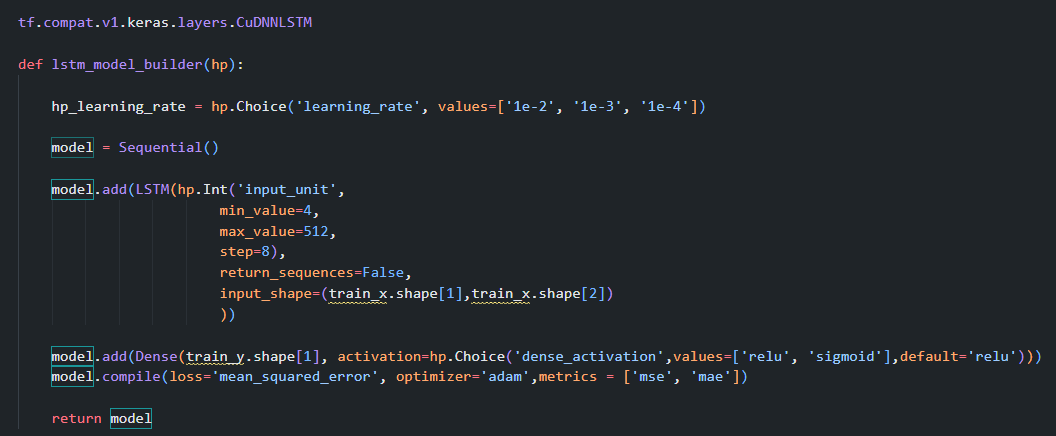
\includegraphics[width=12cm]{../reports/figures/LSTM_model.png}
        \label{LSTM_model_construct}
        \par
        {\small fonte: Produção do próprio autor.}
    \end{figure}

    A ferramenta irá variar a taxa de aprendizagem do modelo, ou seja, 
    quão rápido o modelo convergirá para o mínimo da função de perda.
    Com relação a estrutura da LSTM, será variado a quantidade de unidades LSTM entre 4 e 512 em múltiplos
    de 8 aleatóriamente e por fim, a função de ativação da saída do modelo poderá ser relu (\textit{rectified linear unit}) ou sigmoidal.

    \chapter{Análise dos resultados obtidos}

    Neste capítulo será apresentado os resultados obtidos por cada um dos modelos, realizando uma comparação e
    apontando o modelo que obteve os melhores resultados.

    \begin{itemize}
        \item Modelo de Regressão Linear
    \end{itemize}

    \begin{table}
\centering
\caption{Métricas do modelo de regressão linear}
\label{tab:lin_metrics}
\begin{tabular}{ccc}
\toprule
     rmse &      mae &         mape \\
\midrule
14.922755 & 3.048696 & 4.307988e+14 \\
\bottomrule
\end{tabular}
\end{table}


    Conforme apresentado na Tabela \ref*{tab:lin_metrics} o modelo obteve um RMSE de aproximadamente 15 internações por doenças
    respiratórias, isso significa que, para cada internado o modelo estipulou em média 15 internados a mais ou a menos.
    Esse resultado era esperado, pois foi verificado na Tabela \ref*{corr_table} que não 
    existe correlação linear com a variável de saída.

    A \ref*{scatter_lin_reg} apresenta a relação entre os dados de teste dos valores reais de internações e os valores previstos.

    \begin{figure}[ht]
        \centering
        \caption{Diagrama de dispersão dos dados reais e dos previstos do modelo LR}
        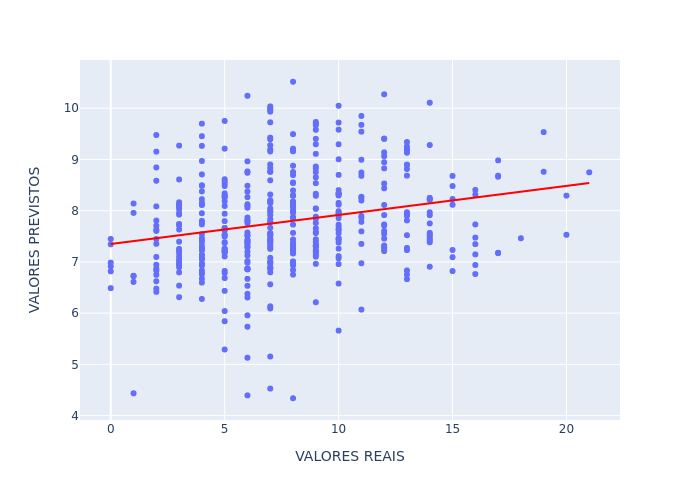
\includegraphics[width=12cm]{../reports/figures/scatter_lin_reg.png}
        \label{scatter_lin_reg}
        \par
        {\small fonte: Produção do próprio autor.}
    \end{figure}

    \begin{itemize}
        \item Árvore de Decisão
    \end{itemize}

    Esse modelo obteve uma grande melhora de performace quando comparado ao modelo de regressão linear, uma das diferenças foi
    a realização da validação cruzada. Observando a tabela \ref*{tab:tree_metrics} nota-se que o RMSE diminuiu 2,74 vezes.


    \begin{table}
\centering
\caption{Métricas do modelo de árvore de decisão}
\label{tab:tree_metrics}
\begin{tabular}{ccc}
\toprule
    rmse &      mae &         mape \\
\midrule
5.344163 & 4.155221 & 2.620422e+14 \\
\bottomrule
\end{tabular}
\end{table}


    A \ref*{scatter_tree_reg} apresenta a relação entre os dados de teste dos valores reais de internações e os valores previstos.

    \begin{figure}[ht]
        \centering
        \caption{Diagrama de dispersão dos dados reais e dos previstos do modelo DT}
        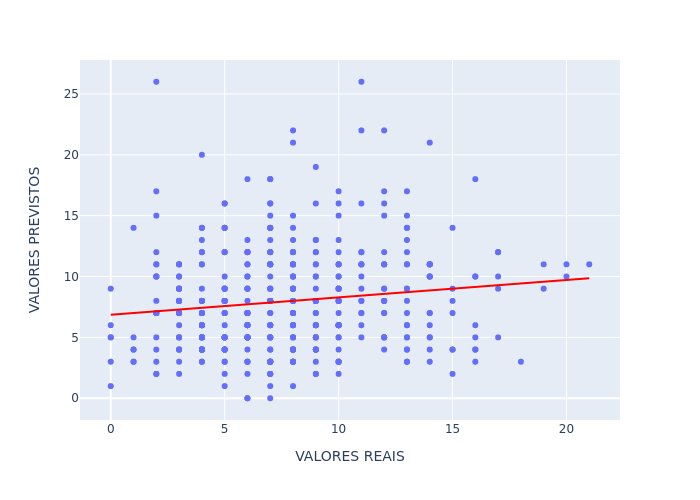
\includegraphics[width=12cm]{../reports/figures/scatter_tree_reg.png}
        \label{scatter_tree_reg}
        \par
        {\small fonte: Produção do próprio autor.}
    \end{figure}

    \begin{itemize}
        \item Floresta Aleatória
    \end{itemize}

    Esse modelo de \textit{machine learning} é o mais robusto dos testados da primeira abordagem, pela tabela \ref*{tab:rf_metrics}
    pode-se concluir que o RF obteve o melhor resultado entre o LR e DT, o RMSE encontrado foi de aproximadamente 4 internados
    a mais ou a menos para cada valor real.

    \begin{table}
\centering
\caption{Métricas do modelo de floresta aleatória}
\label{tab:rf_metrics}
\begin{tabular}{ccc}
\toprule
    rmse &      mae &         mape \\
\midrule
3.952855 & 3.088132 & 2.852175e+14 \\
\bottomrule
\end{tabular}
\end{table}


    A \ref*{scatter_rf_reg} apresenta a relação entre os dados de teste dos valores reais de internações e os valores previstos.

    \begin{figure}[ht]
        \centering
        \caption{Diagrama de dispersão dos dados reais e dos previstos do modelo RF}
        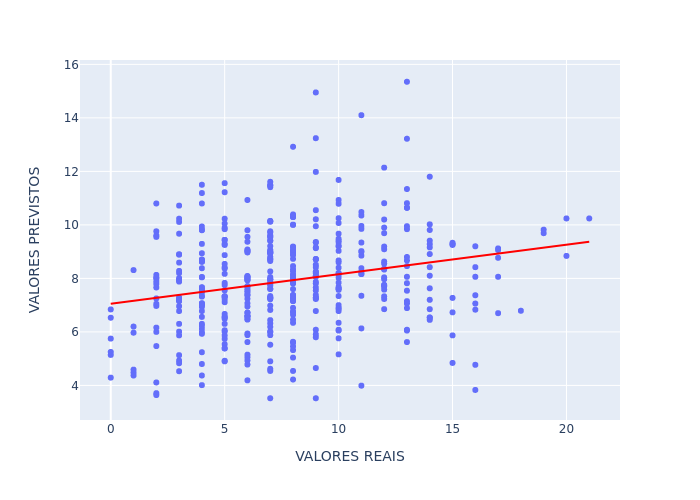
\includegraphics[width=12cm]{../reports/figures/scatter_rf_reg.png}
        \label{scatter_rf_reg}
        \par
        {\small fonte: Produção do próprio autor.}
    \end{figure}

    \begin{itemize}
        \item LSTM
    \end{itemize}

    O modelo de LSTM representa uma grande diferença no tratamento de resolução do problema, pois o trata
    como uma regressão de séries temporais. Isso pode permitir encontrar padrões temporais na
    série que não foram observados nos modelos de \textit{machine learning} descritos anteriormente.

    Analisando a Tabela \ref*{tab:lstm_metrics} percebe-se que o modelo obteve o menor
    RMSE entre todos os modelos testados, isso mostra a robustez de uma rede neural recorrente
    em encontrar padrões não lineares.

    \begin{table}
\centering
\caption{Métricas do modelo LSTM}
\label{tab:lstm_metrics}
\begin{tabular}{ccc}
\toprule
    rmse &      mae &         mape \\
\midrule
3.239208 & 2.720342 & 1.503353e+15 \\
\bottomrule
\end{tabular}
\end{table}


    A \ref*{scatter_lstm_reg} apresenta a relação entre os dados de teste dos valores reais de internações e os valores previstos.

    \begin{figure}[ht]
        \centering
        \caption{Diagrama de dispersão dos dados reais e dos previstos do modelo LSTM}
        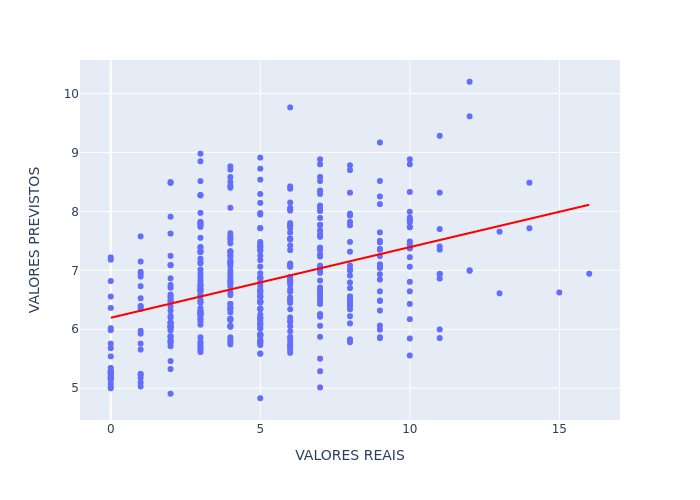
\includegraphics[width=11cm]{../reports/figures/lstm_reg.png}
        \label{scatter_lstm_reg}
        \par
        {\small fonte: Produção do próprio autor.}
    \end{figure}

    A Tabela \ref*{tt} apresenta os resultados obtidos para cada um dos modelos:

    \begin{table}[ht]
        \centering
        \caption{Resultados dos modelos}
        \label{tt}
        \begin{tabular}{cccc}
            \hline
            \multicolumn{1}{|c|}{Modelo} & \multicolumn{1}{c|}{rmse} & \multicolumn{1}{c|}{MAE} & \multicolumn{1}{c|}{MAPE}\\
            \hline
            Regressão Linear & 14.922755 & 3.048696 & 4.307988e+14\\
            Árvore de Decisão & 5.344163 & 4.155221 & 2.620422e+14\\
            Árvore Aleatória & 3.952855 & 3.088132 & 2.852175e+14\\
            LSTM & 3.239208 & 2.720342 & 1.503353e+15\\
            \hline
        \end{tabular}
        \par
        {\small fonte: Adaptado de \cite[]{ibge}}
    \end{table}

    \chapter{Conclusão}

    O principal objetivo desse trabalho foi comparar as técninas de \textit{machine learning} e rede neural artificial apresentadas
    e verificar qual modelo obteve as predições mais próximas dos valores reais observados. 

    Analisando os resultados dos modelos pela métrica MAPE, observa-se que os valores obtidos são extremamente altos. Isso ocorreu, pois muitos valores
    de internações observadas são iguais a 0 e dessa forma, ao calcular esse erro ocorre uma divisão por 0, resultando em valores enormes. Por isso, o MAPE não
    não pode ser levado em consideração na análise.

    Com relação ao erro médio absoluto (MAE) o modelo que obteve a melhor performance foi a LSTM, no entanto, o RF e LR apresentaram erros
    muito próximos, com leve vantagem para a LR. Analisando pela raíz do erro quadrático médio (RMSE), observa-se que o \textit{Random Forest}
    desempenhou desse vez muito melhor que o modelo de regressão linear, isso significa que a LR possuí erros relativamente maiores que o RF. Novamente,
    a LSTM foi o modelo que apresentou o menor erro.

    Dessa forma, tomando como principal métrica de avaliação a raiz do erro quadrático médio (RMSE). 
    O melhor modelo foi um tipo de rede neural recorrente, a \textit{Long Short Term Memory}
    (LSTM). A LSTM foi mais eficaz em encontrar correlações não lineares nos dados de entrada com a variável de saída.

    Assim, diante da problemática apresentada nos capítulos iniciais, conclui-se que esse trabalho contribui para a geração
    de novas informações adequadas que podem ajudar lideres e gestores dos sistemas de saúde da cidade de Cuiabá-MT 
    e de todo o território nacional a traçar estratégias de melhoria dos serviços de saúde e gestão dos recursos, principalmente, 
    mediante um contexto de variações na demanda nos sistemas de saúde. Promovendo, melhor qualidade de vida e 
    condições ao combate das doenças respiratórias.




    \section{PROPOSTAS PARA FUTURAS PESQUISAS}

    \begin{itemize}
        \item Aumentar a base de dados;
        \item Analisar a influência das \textit{features} não utilizadas, variando-as na base de dados;
        \item Analisar a influência da utilização de diferentes \textit{lags}, variando entre 0 a 7;
        \item Realizar \textit{Hyperparameter boost} da \textit{Random Forest};
        \item Utilizar outros modelos de \textit{machine learning} como XGboost e SVR;
        \item Aumentar a complexidade do modelo de LSTM.
    \end{itemize}
    %------------------------------------------------------------------------------------%
    %                               P Ó S   T E X T U A L                                %
    %                                                                                    %
    % Fim do corpo do texto. A partir desse comando as indicações no sumário serão       %
    % marcadas como 'pós textuais'.                                                      %
    %------------------------------------------------------------------------------------%
    
    \postextual
    
    %------------------------------------------------------------------------------------%
    % R E F E R Ê N C I A S
    %
    % OBRIGATÓRIO. Será gerada automaticamente a partir do arquivo "references.bib".
    %------------------------------------------------------------------------------------%
    
    \bibliography{references}
    
    %------------------------------------------------------------------------------------%
    % A P Ê N D I C E S
    %
    % OPCIONAL. Consiste em um texto ou documento elaborado pelo autor a fim de complementar
    % sua argumentação. Se necessário ter mais de um apêndice, basta adicionar cada um dentro
    % de um dentro de um comando "\chapter". % Se não for utilizar um Apêndice, basta apagar
    % todo o código dessa seção.
    %------------------------------------------------------------------------------------%
    
    % \begin{apendicesenv}
        
    %     \chapter{Título do Apêndice A}
    %         \lipsum[50]
        
    %     \chapter{Título do Apêndice B}
    %         \lipsum[51]
        
    % \end{apendicesenv}
    
    %------------------------------------------------------------------------------------%
    % A N E X O S
    %
    % OPCIONAL. Consiste em um texto ou documento não elaborado pelo autor que serve de
    % fundamentação, comprovação ou ilustração ao trabalho. Se necessário ter mais de um
    % anexo, basta adicionar cada um dentro de um dentro de um comando "\chapter".
    % Se não for utilizar nenhum Anexo, basta apagar todo o código dessa seção.
    %------------------------------------------------------------------------------------%
    
    % \begin{anexosenv}
    
    %     \chapter{Título do Anexo A}
    %         \lipsum[30]
      
    %     \chapter{Título do Anexo B}
    %         \lipsum[31]
        
    %     \chapter{Título do Anexo C}
    %         \lipsum[32]
      
    % \end{anexosenv}
    
\end{document}

